% Options for packages loaded elsewhere
\PassOptionsToPackage{unicode}{hyperref}
\PassOptionsToPackage{hyphens}{url}
\documentclass[
  12pt,
]{article}
\usepackage{xcolor}
\usepackage[margin=2.5cm]{geometry}
\usepackage{amsmath,amssymb}
\setcounter{secnumdepth}{5}
\usepackage{iftex}
\ifPDFTeX
  \usepackage[T1]{fontenc}
  \usepackage[utf8]{inputenc}
  \usepackage{textcomp} % provide euro and other symbols
\else % if luatex or xetex
  \usepackage{unicode-math} % this also loads fontspec
  \defaultfontfeatures{Scale=MatchLowercase}
  \defaultfontfeatures[\rmfamily]{Ligatures=TeX,Scale=1}
\fi
\usepackage{lmodern}
\ifPDFTeX\else
  % xetex/luatex font selection
  \setmainfont[]{TeX Gyre Termes}
\fi
% Use upquote if available, for straight quotes in verbatim environments
\IfFileExists{upquote.sty}{\usepackage{upquote}}{}
\IfFileExists{microtype.sty}{% use microtype if available
  \usepackage[]{microtype}
  \UseMicrotypeSet[protrusion]{basicmath} % disable protrusion for tt fonts
}{}
\makeatletter
\@ifundefined{KOMAClassName}{% if non-KOMA class
  \IfFileExists{parskip.sty}{%
    \usepackage{parskip}
  }{% else
    \setlength{\parindent}{0pt}
    \setlength{\parskip}{6pt plus 2pt minus 1pt}}
}{% if KOMA class
  \KOMAoptions{parskip=half}}
\makeatother
\usepackage{color}
\usepackage{fancyvrb}
\newcommand{\VerbBar}{|}
\newcommand{\VERB}{\Verb[commandchars=\\\{\}]}
\DefineVerbatimEnvironment{Highlighting}{Verbatim}{commandchars=\\\{\}}
% Add ',fontsize=\small' for more characters per line
\usepackage{framed}
\definecolor{shadecolor}{RGB}{248,248,248}
\newenvironment{Shaded}{\begin{snugshade}}{\end{snugshade}}
\newcommand{\AlertTok}[1]{\textcolor[rgb]{0.94,0.16,0.16}{#1}}
\newcommand{\AnnotationTok}[1]{\textcolor[rgb]{0.56,0.35,0.01}{\textbf{\textit{#1}}}}
\newcommand{\AttributeTok}[1]{\textcolor[rgb]{0.13,0.29,0.53}{#1}}
\newcommand{\BaseNTok}[1]{\textcolor[rgb]{0.00,0.00,0.81}{#1}}
\newcommand{\BuiltInTok}[1]{#1}
\newcommand{\CharTok}[1]{\textcolor[rgb]{0.31,0.60,0.02}{#1}}
\newcommand{\CommentTok}[1]{\textcolor[rgb]{0.56,0.35,0.01}{\textit{#1}}}
\newcommand{\CommentVarTok}[1]{\textcolor[rgb]{0.56,0.35,0.01}{\textbf{\textit{#1}}}}
\newcommand{\ConstantTok}[1]{\textcolor[rgb]{0.56,0.35,0.01}{#1}}
\newcommand{\ControlFlowTok}[1]{\textcolor[rgb]{0.13,0.29,0.53}{\textbf{#1}}}
\newcommand{\DataTypeTok}[1]{\textcolor[rgb]{0.13,0.29,0.53}{#1}}
\newcommand{\DecValTok}[1]{\textcolor[rgb]{0.00,0.00,0.81}{#1}}
\newcommand{\DocumentationTok}[1]{\textcolor[rgb]{0.56,0.35,0.01}{\textbf{\textit{#1}}}}
\newcommand{\ErrorTok}[1]{\textcolor[rgb]{0.64,0.00,0.00}{\textbf{#1}}}
\newcommand{\ExtensionTok}[1]{#1}
\newcommand{\FloatTok}[1]{\textcolor[rgb]{0.00,0.00,0.81}{#1}}
\newcommand{\FunctionTok}[1]{\textcolor[rgb]{0.13,0.29,0.53}{\textbf{#1}}}
\newcommand{\ImportTok}[1]{#1}
\newcommand{\InformationTok}[1]{\textcolor[rgb]{0.56,0.35,0.01}{\textbf{\textit{#1}}}}
\newcommand{\KeywordTok}[1]{\textcolor[rgb]{0.13,0.29,0.53}{\textbf{#1}}}
\newcommand{\NormalTok}[1]{#1}
\newcommand{\OperatorTok}[1]{\textcolor[rgb]{0.81,0.36,0.00}{\textbf{#1}}}
\newcommand{\OtherTok}[1]{\textcolor[rgb]{0.56,0.35,0.01}{#1}}
\newcommand{\PreprocessorTok}[1]{\textcolor[rgb]{0.56,0.35,0.01}{\textit{#1}}}
\newcommand{\RegionMarkerTok}[1]{#1}
\newcommand{\SpecialCharTok}[1]{\textcolor[rgb]{0.81,0.36,0.00}{\textbf{#1}}}
\newcommand{\SpecialStringTok}[1]{\textcolor[rgb]{0.31,0.60,0.02}{#1}}
\newcommand{\StringTok}[1]{\textcolor[rgb]{0.31,0.60,0.02}{#1}}
\newcommand{\VariableTok}[1]{\textcolor[rgb]{0.00,0.00,0.00}{#1}}
\newcommand{\VerbatimStringTok}[1]{\textcolor[rgb]{0.31,0.60,0.02}{#1}}
\newcommand{\WarningTok}[1]{\textcolor[rgb]{0.56,0.35,0.01}{\textbf{\textit{#1}}}}
\usepackage{longtable,booktabs,array}
\usepackage{calc} % for calculating minipage widths
% Correct order of tables after \paragraph or \subparagraph
\usepackage{etoolbox}
\makeatletter
\patchcmd\longtable{\par}{\if@noskipsec\mbox{}\fi\par}{}{}
\makeatother
% Allow footnotes in longtable head/foot
\IfFileExists{footnotehyper.sty}{\usepackage{footnotehyper}}{\usepackage{footnote}}
\makesavenoteenv{longtable}
\usepackage{graphicx}
\makeatletter
\newsavebox\pandoc@box
\newcommand*\pandocbounded[1]{% scales image to fit in text height/width
  \sbox\pandoc@box{#1}%
  \Gscale@div\@tempa{\textheight}{\dimexpr\ht\pandoc@box+\dp\pandoc@box\relax}%
  \Gscale@div\@tempb{\linewidth}{\wd\pandoc@box}%
  \ifdim\@tempb\p@<\@tempa\p@\let\@tempa\@tempb\fi% select the smaller of both
  \ifdim\@tempa\p@<\p@\scalebox{\@tempa}{\usebox\pandoc@box}%
  \else\usebox{\pandoc@box}%
  \fi%
}
% Set default figure placement to htbp
\def\fps@figure{htbp}
\makeatother
% definitions for citeproc citations
\NewDocumentCommand\citeproctext{}{}
\NewDocumentCommand\citeproc{mm}{%
  \begingroup\def\citeproctext{#2}\cite{#1}\endgroup}
\makeatletter
 % allow citations to break across lines
 \let\@cite@ofmt\@firstofone
 % avoid brackets around text for \cite:
 \def\@biblabel#1{}
 \def\@cite#1#2{{#1\if@tempswa , #2\fi}}
\makeatother
\newlength{\cslhangindent}
\setlength{\cslhangindent}{1.5em}
\newlength{\csllabelwidth}
\setlength{\csllabelwidth}{3em}
\newenvironment{CSLReferences}[2] % #1 hanging-indent, #2 entry-spacing
 {\begin{list}{}{%
  \setlength{\itemindent}{0pt}
  \setlength{\leftmargin}{0pt}
  \setlength{\parsep}{0pt}
  % turn on hanging indent if param 1 is 1
  \ifodd #1
   \setlength{\leftmargin}{\cslhangindent}
   \setlength{\itemindent}{-1\cslhangindent}
  \fi
  % set entry spacing
  \setlength{\itemsep}{#2\baselineskip}}}
 {\end{list}}
\usepackage{calc}
\newcommand{\CSLBlock}[1]{\hfill\break\parbox[t]{\linewidth}{\strut\ignorespaces#1\strut}}
\newcommand{\CSLLeftMargin}[1]{\parbox[t]{\csllabelwidth}{\strut#1\strut}}
\newcommand{\CSLRightInline}[1]{\parbox[t]{\linewidth - \csllabelwidth}{\strut#1\strut}}
\newcommand{\CSLIndent}[1]{\hspace{\cslhangindent}#1}
\setlength{\emergencystretch}{3em} % prevent overfull lines
\providecommand{\tightlist}{%
  \setlength{\itemsep}{0pt}\setlength{\parskip}{0pt}}
\usepackage{setspace}\doublespacing
\setstretch{1.5}
\usepackage{parskip}
\setlength{\parskip}{6pt}
\setlength{\parindent}{0pt}
\usepackage{float}
\usepackage{longtable}
\newcommand{\argmin}{\mathop{\mathrm{argmin}}\limits}
\usepackage{booktabs}
\usepackage{longtable}
\usepackage{array}
\usepackage{multirow}
\usepackage{wrapfig}
\usepackage{float}
\usepackage{colortbl}
\usepackage{pdflscape}
\usepackage{tabu}
\usepackage{threeparttable}
\usepackage{threeparttablex}
\usepackage[normalem]{ulem}
\usepackage{makecell}
\usepackage{xcolor}
\usepackage{bookmark}
\IfFileExists{xurl.sty}{\usepackage{xurl}}{} % add URL line breaks if available
\urlstyle{same}
\hypersetup{
  pdftitle={The Foreign Policy Impact of Trade-Based Status Gains: When China Overtakes the US as Top Export Destination},
  pdfauthor={Manoel Galdino (University of São Paulo; mgaldino@usp.br)},
  hidelinks,
  pdfcreator={LaTeX via pandoc}}

\title{The Foreign Policy Impact of Trade-Based Status Gains: When China Overtakes the US as Top Export Destination}
\author{Manoel Galdino (University of São Paulo; \href{mailto:mgaldino@usp.br}{\nolinkurl{mgaldino@usp.br}})}
\date{2026-08-27}

\begin{document}
\maketitle
\begin{abstract}
\singlespacing  How do trade-based status gains affect UNGA voting convergence toward China? I argue that rank reversals in trade hierarchies create politically usable status cues: when China becomes a country's top export destination and remains there, policymakers can more easily justify selective diplomatic adjustment toward Beijing. I test the argument in Brazil, where China overtook the United States as the largest export destination in 2009, using Synthetic Difference-in-Differences on UNGA ideal-point distance. In the preferred specification, the estimated effect is a reduction of 0.27 ideal-point units in Brazil's distance to China relative to its synthetic counterfactual, about 42 percent of Brazil's pre-treatment mean. Vote-level diagnostics show that the movement is clearest in human-rights resolutions where China and the United States diverged. Brazilian newspaper evidence shows increased China-related trade salience after the rank reversal. Cross-country estimates from an interactive fixed-effects panel model show a compatible directional pattern among countries where China persistently becomes the top goods export destination. The evidence suggests that discrete and durable trade-status milestones can shape observable multilateral alignment beyond smooth trade growth.
\end{abstract}

\pagebreak

Word count: 14,539

\section{Introduction}\label{introduction}

``China overtakes US as Brazil's top trade partner''. That was a headline in many Brazilian newspapers in 2009 (\citeproc{ref-rodrigues2009}{A. Rodrigues 2009}). The BBC ran a similar headline in 2021, when China surpassed the United States as the EU's biggest trading partner (\citeproc{ref-bbc2021}{BBC News 2021}). During a high-profile trip to Beijing with an unusually large business delegation, President Lula da Silva invoked the milestone by noting that China was Brazil's largest export destination (\citeproc{ref-lula2009}{Presidência da República Federativa do Brasil 2009}).

Why do media outlets and political leaders dwell on discrete commercial milestones when the underlying flows are measured continuously? Export statistics are updated monthly, and journalists, diplomats, firms, and policymakers follow them long before one partner crosses a formal threshold. The puzzle, then, is not whether actors possess information about trade volumes. It is why a categorical change -- China becomes number one -- can matter politically despite adding little new information about the economic trend itself.

Answering this question rigorously is difficult because trade hierarchies are not randomly assigned. Existing work on economic statecraft and foreign-policy alignment usually treats economic exposure as continuous: as trade, lending, investment, aid, or coercive capacity accumulate, alignment is expected to shift through material leverage, changing interests, soft power, or domestic pressure (\citeproc{ref-flores-macias_kreps2013}{Flores-Macías and Kreps 2013}; \citeproc{ref-urdinez_etal2016}{Urdinez et al. 2016}; \citeproc{ref-kastner_pearson2021}{Kastner and Pearson 2021}). A continuous-interdependence account would therefore expect foreign-policy alignment to move gradually with trade exposure, leverage, and economic dependence rather than at a discrete rank threshold. Domestic-political accounts, by contrast, would attribute foreign-policy change in cases such as Brazil to leadership ideology, autonomy, South-South cooperation, or broader foreign-policy reorientation (\citeproc{ref-neto2011}{Neto 2011}; \citeproc{ref-neto_malamud2015}{Neto and Malamud 2015}; \citeproc{ref-rodrigues2019measuring}{P. Rodrigues, Urdinez, and De Oliveira 2019}; \citeproc{ref-schenoniMythsMultipolaritySources2022}{Luis L. Schenoni et al. 2022}). A further selection concern is that politically aligned countries may deepen economic ties with one another, making China's rise in the trade hierarchy a consequence rather than a cause of prior diplomatic affinity (\citeproc{ref-gowa1995}{Gowa 1995}; \citeproc{ref-davis_pratt2021}{Davis and Pratt 2021}; \citeproc{ref-struver2016}{Strüver 2016}). If alignment reflects only accumulated exposure, domestic-political reorientation, or prior diplomatic affinity, however, no specific symbolic milestone such as becoming a top trade partner should matter.

I argue that such milestones matter because they mark trade-based status gains. The argument builds on research that treats status as socially recognized standing within international hierarchies, clubs, and local status orders (\citeproc{ref-paul_larson_wohlforth2014}{Paul, Larson, and Wohlforth 2014}; \citeproc{ref-wolfRespectDisrespect2011}{Wolf 2011}, \citeproc{ref-wolfTakingInteractionSeriously2019}{2019}; \citeproc{ref-duque_2018}{Duque 2018}; \citeproc{ref-renshon2017}{Renshon 2017}; \citeproc{ref-gotz_2021}{Götz 2021}; \citeproc{ref-macdonald_parent2021}{MacDonald and Parent 2021}; \citeproc{ref-roren_2024}{Røren 2024}, \citeproc{ref-roren2025_power_recognition}{2025}). By trade-based status, I mean the recognized standing of a foreign power within a country's hierarchy of economically consequential relationships. Trade volume is continuous, but status is categorical: a partner can move from being important to being understood as central. Once that reclassification becomes public, the relationship is no longer merely larger than before. It becomes easier for political actors to invoke as a national priority, to defend as strategically consequential, and to use as a justification for diplomatic adjustment.

Much of the China and rising-powers branch of this literature asks how rising states seek recognition, major-power status, or institutional standing, and how misrecognition can produce contestation or revisionism (\citeproc{ref-deng2008_status}{Deng 2008}; \citeproc{ref-larson_shevchenko2010_status_seekers}{Larson and Shevchenko 2010}; \citeproc{ref-ward2017_status_challenge}{Ward 2017}; \citeproc{ref-murray2018_recognition}{Murray 2018}; \citeproc{ref-mukherjee2022_ascending}{Mukherjee 2022}). This argument relocates status from the ambitions of the rising power to the recognition practices of states. China's trade-based status gain occurs when another country publicly recategorizes China within its own hierarchy of external economic relationships -- from an important partner to a central one. The mechanism is therefore status-theoretic, with Brazil as the audience and status-conferring actor.

Brazil is the strongest case for the theory. Firstly, China displaced the United States, a politically salient incumbent, hegemonic benchmark and the most important trade partner of Brazil for almost 80 years. Secondly, the rank reversal was publicly visible. And thirdly, the Brazilian press allows the attention implication to be measured. The case is also substantively important because Lula-era Brazilian foreign policy is often described through autonomy, South-South activism, multipolarity, and Brazil's triangular position between the United States and China (\citeproc{ref-neto2011}{Neto 2011}; \citeproc{ref-neto_malamud2015}{Neto and Malamud 2015}; \citeproc{ref-rodrigues2019measuring}{P. Rodrigues, Urdinez, and De Oliveira 2019}; \citeproc{ref-schenoniMythsMultipolaritySources2022}{Luis L. Schenoni et al. 2022}; \citeproc{ref-guilhon2014}{Guilhon-Albuquerque 2014}; \citeproc{ref-schenoni_leiva2021}{Luis L. Schenoni and Leiva 2021}; \citeproc{ref-brun_covarrubias2024}{Brun and Covarrubias 2024}; \citeproc{ref-coutinho_rodriguez2024}{Coutinho and Rodriguez 2024}).

To estimate the Brazilian foreign-policy alignment pattern, I use synthetic difference-in-differences (SDiD) on annual UNGA ideal-point distance to China, with 2009 marking China's rise to the largest Brazilian export destination. UNGA voting is a standard measure to study alignment with China and other powers, linking votes to bilateral ties, ideology, sanctions, aid, Belt and Road membership, arms transfers, or Chinese economic returns (\citeproc{ref-potrafke2009}{Potrafke 2009}; \citeproc{ref-dreher_jensen2013}{Dreher and Jensen 2013}; \citeproc{ref-struver2016}{Strüver 2016}; \citeproc{ref-yan_zhou2021}{Yan and Zhou 2021}; \citeproc{ref-garcia_herrero_etal2024}{Garcia-Herrero, Storella, and Weil 2024}; \citeproc{ref-steinert_weyrauch2024}{Steinert and Weyrauch 2024}; \citeproc{ref-he_zheng_chen2025}{He, Zheng, and Chen 2025}; \citeproc{ref-lektzian_biglaiser2023}{Lektzian and Biglaiser 2023}).

In the preferred specification, the estimated effect is a reduction of 0.273 ideal-point units in Brazil's distance to China relative to its synthetic counterfactual, equivalent to 42.2 percent of its pre-treatment mean, with a one-sided placebo-rank p-value of 0.031.

To assess whether the pattern is specific to Brazil and check potential confound threats to a causal interpretation of the findings, I extend the analysis to a cross-country panel in which China enters and holds the top goods export-destination position. The cross-country estimates are smaller in magnitude, consistent with a more heterogeneous sample, and point in the same direction as the Brazilian case. The pooled panel estimate is -0.101 (p-value = 0.010) and is stable across duration thresholds and sample restrictions (p-value between 0.003 and 0.019). The panel evidence is compatible with the rank-threshold argument beyond the theory-generating case, while the Brazilian evidence documents the mechanism in detail.

The paper's contribution is to recast economic influence as a status process. Existing work usually treats trade exposure as a continuous source of leverage, interests, or domestic pressure. I show that accumulated trade growth can become politically consequential when it crosses a durable, publicly legible rank threshold: when China becomes and remains a country's largest export destination, the new status condition creates a persistent basis for selective diplomatic adjustment. In Brazil, China's rise to the top export-destination position made an already expanding commercial relationship politically usable as evidence of China's new centrality. That status gain helps explain why convergence appears selectively in UNGA voting. More broadly, the paper shows that status gains can emerge from economic hierarchies and shape observable diplomatic behavior.

The next section develops the status-threshold argument and derives observable implications. I then present the Brazil SDiD design and timing diagnostics, followed by issue-area and media evidence on the mechanism. The final empirical section evaluates whether durable China-top goods-export status is associated with similar movement in a broader cross-country panel.

\section{Theory and hypotheses}\label{theory-and-hypotheses}

A trade-based status shift differs from smooth growth in economic interdependence because it changes the category through which a foreign power is understood. Actors can observe trade shares, but political attention rarely follows continuous movements one percentage point at a time. It also organizes around coarse public labels: largest export market, number-one partner, top-ranked export destination. These labels simplify complex economic relationships and help journalists, politicians, organized interests, and diplomats coordinate attention (\citeproc{ref-bordalo_etal2022}{Bordalo, Gennaioli, and Shleifer 2022}; \citeproc{ref-conlon2023}{Conlon 2025}; \citeproc{ref-enke2024}{Enke 2024}; \citeproc{ref-graeber_etal2025}{Graeber, Roth, and Sammon 2025}). The number-one threshold matters because it can reclassify a rising power from one important commercial partner among several into the country's central economic partner. In this sense, export-destination rank operationalizes the trade-based status shift.

The cue should matter most when the new status also displaces a politically prominent incumbent. If a rising major power overtakes a minor partner, the event may remain a commercial fact with limited political resonance. If it overtakes the hegemonic incumbent, the same threshold takes on broader political meaning. It can be read as a visible loss of standing for the incumbent and as a public marker of the challenger's rise. Brazil falls squarely inside this high-salience condition: China became Brazil's largest export destination in 2009, displaced the United States, and contemporary coverage frequently described the event in broader top-partner language.

The mechanism has two steps. First, the status cue should increase attention. Media coverage should make the challenger and the bilateral trade relationship more visible after the threshold is crossed. Second, the cue should affect policy through justification. Once that power is publicly understood as a central economic partner, executives and diplomats can frame limited movement toward it as pragmatic recognition of the country's economic hierarchy rather than as ideological concession or opportunistic bandwagoning. This step can be gradual because UNGA positions are embedded in prior votes, bureaucratic routines, coalition commitments, and reputational constraints. The Brazilian SDiD design estimates the combined reduced-form effect of this status cue on UNGA distance to China.

The justification mechanism also implies a durability condition. The rank reversal is not expected to reshape foreign policy through a single decision at the moment China becomes number one. Rather, it creates a public category that officials can invoke repeatedly across a sequence of selective adjustments. When China remains the largest export destination, presidents, ministers, diplomats, and organized interests can treat its centrality as a stable fact of the national economic hierarchy and use it to justify incremental diplomatic movement. A one-year China-top episode may attract attention, but it is a weaker treatment regime: it does not provide a durable basis for repeated public justification, bureaucratic recalibration, or cumulative foreign-policy adaptation.

\subsection{From Attention to Selective Diplomatic Alignment}\label{from-attention-to-selective-diplomatic-alignment}

Trade-based status changes the terms on which selective accommodation can be justified. Some foreign-policy arenas are especially suitable for this kind of adjustment: they are visible to foreign governments and diplomatic audiences, materially less costly than treaties, military commitments, sanctions, or trade policy, and still capable of generating reputational exposure. In such arenas, governments can signal movement toward a newly central partner while preserving flexibility.

When a foreign power's rise to the top export-destination position is publicly recognized as evidence of centrality in the country's trade hierarchy, policymakers can frame limited convergence with that power as pragmatic recognition of economic importance rather than as ideological concession or opportunistic bandwagoning. The status gain can therefore lower the reputational cost of selected movement while increasing its diplomatic value.

The domestic pathway works through justification. Media coverage need not cause individual foreign-policy positions, and business groups need not lobby over specific diplomatic decisions. Public recognition of the partner's new standing changes what diplomats and executives can plausibly defend. Adjustment toward that partner becomes easier to present as alignment with national economic interests, especially in diplomatic settings where positions are visible internationally but relatively low-cost domestically.

This logic implies selective convergence. The mechanism should be most informative in issue areas where the country and the newly elevated partner previously differed and where movement is not costless. In domains tied to prior reputational commitments, adjustment toward the newly central partner requires a stronger rationale than in areas where the two countries already agree. Trade-based status supplies such a rationale by making the partner's economic centrality publicly available as a justification for diplomatic accommodation.

The main theoretical expectation is therefore that when a rising major power becomes a country's largest export destination and that milestone becomes a public trade-status cue, the country's foreign policy should move closer to that power relative to its counterfactual path. The effect should be easiest to observe when the status gain displaces a politically prominent incumbent, especially a hegemonic benchmark such as the United States. The theory also implies an attention pattern: media coverage of the rising power and of the bilateral economic relationship should increase around the status shift.

\section{Data and design}\label{data-and-design}

The theoretical concept of interest is the rising power obtaining the status of top trade partner of a country. However, public status language varies in what counts as a top trade partner and in how it is described. Officials and journalists may describe China as the largest trading partner, main commercial partner, or top export market, for instance. Countries also value different things as a matter of status: largest flow of trade (exports plus imports) is what matters for some countries. For others, it is largest total exports (goods and services), or largest goods exports.

For the argument advanced in the article, what matters is the status change. In practice, the design uses specifically an export-destination rank -- to become number one in that rank. In Brazil, public and official language tracks that rank: the 2009 coverage announcing that China had overtaken the United States as the country's largest trading partner was reporting precisely that change. Elsewhere the same phrase may track aggregate flows, including imports and services, which is a source of measurement error in the cross-country panel.

A supplemental source audit in the appendix uses displaced-incumbent coverage to check evidence of coverage in other countries. Australia illustrates the point. The \emph{Australian Financial Review} reported in 2009 that China was Australia's largest aggregate trading partner, combining exports and imports of goods and services, before Australia meets the paper's stricter goods-export-destination treatment criterion. As a result, in the panel regression with other treated countries besides Brazil, there is error in the measurement of the treatment.

The primary outcome is absolute UNGA ideal-point distance to China, based on the annual ideal-point estimates of Bailey, Strezhnev, and Voeten (\citeproc{ref-bailey_etal2017}{2017}). Lower values indicate convergence toward China. This measure is preferable to raw annual agreement shares for the main design because it is less sensitive to changes in the UNGA agenda over time. I use resolution-level agreement diagnostics only to interpret where convergence appears strongest. As a measurement-robustness check, the appendix re-estimates the main specifications using ideal points estimated by Fjelstul, Hug, and Kilby (\citeproc{ref-fjelstul_etal2026}{2026}), which are slightly different from Bailey, Strezhnev, and Voeten (\citeproc{ref-bailey_etal2017}{2017}) and based on another sample of resolution-related votes.

For Brazil, the treatment indicator equals one from 2009 onward, the first year China became Brazil's largest export destination. SDiD estimates Brazil's average post-2009 gap relative to a weighted synthetic counterfactual, using pre-treatment information to construct unit and time weights (\citeproc{ref-arkhangelsky_etal2021}{Arkhangelsky et al. 2021}). The design is reduced-form. Its credibility rests on pre-treatment fit, rank-versus-volume timing tests, donor-pool sensitivity, and outcome robustness.

The SDiD panel combines UNGA ideal points with trade, macroeconomic, power, geographic, institutional, and trade-agreement variables. The complete panel covers 96 countries and 19 Brazil years for the main SDiD window (1997-2015). The preferred estimator uses no covariates: the counterfactual is built from pre-treatment outcomes together with the SDiD unit and time weights. Time-varying variables enter only comparison specifications. Trade data come from the International Trade and Production Database for Estimation (\citeproc{ref-borchert_etal2021}{Borchert et al. 2021}). The ITPD-E \texttt{trade} variable is measured in millions of current US dollars, and export-destination ranks are computed from exporter-importer flows.

The Brazil variables enter the design in three groups. The outcome is Brazil's annual absolute UNGA ideal-point distance to China; the treatment is an indicator for years after China becomes Brazil's largest export destination; and observed country characteristics are used for diagnostics and comparison specifications. The preferred counterfactual is driven by pre-treatment outcomes and SDiD unit and time weights, not by effective covariate adjustment. Contemporaneous trade, macroeconomic, power, ideology, and institutional measures remain available for comparisons but are not preferred because their post-2009 values may be mediators or outcomes of the same shocks. The cross-country panel uses the same outcome but constructs treatment separately from goods-only export-destination ranks and a status-current risk set. Table \ref{tab:table-summary-main} summarizes the full country-year panel from which the Brazil specifications are constructed.

\begin{table}[H]
\centering
\caption{\label{tab:table-summary-main}Descriptive statistics for the country-year panel used in the Brazil SDiD design.}
\centering
\resizebox{\ifdim\width>\linewidth\linewidth\else\width\fi}{!}{
\fontsize{8}{10}\selectfont
\begin{threeparttable}
\begin{tabular}[t]{lccccc}
\toprule
Variable & N & Mean & SD & Min & Max\\
\midrule
Treatment & 1824 & 0.00 & 0.06 & 0.00 & 1.00\\
UNGA distance to China & 1824 & 0.91 & 0.80 & 0.00 & 4.22\\
UNGA distance to US & 1824 & 2.65 & 0.92 & 0.00 & 5.06\\
Geographic distance to US & 1824 & 0.00 & 0.50 & -1.14 & 1.11\\
Trade share with China & 1824 & -0.01 & 0.49 & -0.36 & 4.96\\
\addlinespace
Trade share with US & 1824 & 0.00 & 0.50 & -0.41 & 1.87\\
Power index & 1824 & 0.00 & 0.50 & -0.12 & 5.01\\
Power gap to US & 1824 & 0.03 & 0.49 & -3.90 & 0.43\\
GDP per capita & 1824 & -0.00 & 0.50 & -0.37 & 2.81\\
Exchange rate & 1824 & -0.00 & 0.49 & -0.15 & 6.82\\
\addlinespace
HoG left ideology & 1824 & 0.40 & 0.49 & 0.00 & 1.00\\
Current account & 1824 & 0.00 & 0.50 & -3.24 & 2.56\\
Government deficit & 1824 & 0.01 & 0.50 & -6.59 & 3.33\\
Parliamentary system & 1824 & 0.39 & 0.49 & 0.00 & 1.00\\
Military executive & 1824 & 0.11 & 0.31 & 0.00 & 1.00\\
\addlinespace
US trade agreement & 1824 & 0.09 & 0.28 & 0.00 & 1.00\\
\bottomrule
\end{tabular}
\begin{tablenotes}
\item \textit{Note: } 
\item Country-year variables from the SDiD analytic panel; continuous covariates are rescaled in the estimation data, UNGA distances are ideal-point distances, and treatment is binary. Window: 1997-2015 SDiD analytic panel. Observations include Brazil and donor countries used to construct the synthetic counterfactual. The treatment mean is small because only Brazil is treated after 2009. Covariate summaries describe the full analytic panel; the preferred estimate uses none of them.
\end{tablenotes}
\end{threeparttable}}
\end{table}

For the cross-country evidence beyond Brazil, the main sample is restricted to durable China-top export-destination periods measured with goods exports only. The treatment equals one only in country-years where China is the largest goods export destination and that China-top period lasts at least five observed years in the joint trade-rank and UNGA-outcome panel. Treated countries must first enter this status in or after 2000, after an observed prior year in which China was not number one. Countries that never reach China-top goods-export status remain controls. For treated countries, the main risk set keeps clean pre-entry non-China-top years and qualifying treated years, while excluding post-exit off-status years and short China-top episodes. This operationalization matches the salience logic more closely than either a one-year entry definition or an absorbing treatment rule: the theory expects political visibility, bureaucratic learning, and diplomatic adaptation to be clearer when the new trade hierarchy persists and is currently true. I compute partner ranks from ITPD-E goods sectors only, excluding services before ranks are constructed. For this panel, I use the \texttt{fect} counterfactual estimator with interactive fixed effects, which allows countries to load differently on common latent shocks (\citeproc{ref-liu2024practical}{Liu, Wang, and Xu 2024}). I refer to this as the IFE specification below.

\subsection{Identification strategy}\label{identification-strategy}

The empirical problem is that China's rise in a country's trade hierarchy is not randomly assigned. Countries may move closer to China because trade exposure accumulates continuously, because domestic political coalitions or foreign-policy doctrines change, or because governments already inclined toward China deepen commercial ties before the rank reversal occurs.

In the Brazil design, SDiD constructs a weighted counterfactual from pre-treatment outcomes. The preferred specification uses no covariates because time-varying post-2009 values may be affected by the rank reversal, the commodity cycle, or contemporaneous domestic responses. A model specification with time-varying variables uses contemporaneous matrix of trade, power, ideology, macroeconomic stress, and institutional variables. The similarity of the estimates is informative about sensitivity to post-treatment adjustment, but the contemporaneous specification is not the preferred total-effect estimand. Commodity composition and price interactions are also treated as robustness or mechanism diagnostics, especially because the 2008--2009 interaction includes the first treated year.

To compute the uncertainty of estimates, I use a one-sided placebo-in-space rank of the Brazil estimate within the distribution of placebo estimates obtained by reassigning treatment to each unit from the donor pool. For robustness, I also report the standard error calculated from the normal approximation native to the SDiD estimator. I use a one-sided hypothesis test, since the theory is directional (a treated unit should move its ideal point toward China), and report the two-sided test as a conservative sensitivity assessment.

Two features of rank-based inference with a single treated unit are noteworthy. First, with 96 countries, the best case scenario would be for Brazil to present the biggest effect and be the number one over 96 (approximately 0.010), so rank p-values move in coarse steps and have a floor of about 1 percent. Second, the two-sided absolute rank counts large placebo effects of either sign against Brazil, including positive placebo effects that do not represent the error relevant to a directional hypothesis. That is why I call it a conservative assessment of the uncertainty. To be consistent, I apply the same convention uniformly to every placebo-based diagnostic in the paper, including the vote-level human-rights benchmark.

The cross-country panel provides a second check against Brazil-specific timing explanations. Treated countries enter durable China-top goods-export status in different years, so a Brazil-specific 2009 shock cannot mechanically generate the pooled result. Interactive fixed effects allow countries to load differently on common latent shocks, while the appendix reports duration-threshold and risk-set robustness checks.

\section{Brazil SDiD evidence}\label{brazil-sdid-evidence}

The Brazilian analysis estimates the average post-2009 reduced-form effect of China's entry into the top export-destination position on Brazil's UNGA ideal-point distance to China. It asks whether Brazil moved closer to China than a synthetic counterfactual after the 2009 rank reversal.

Figure \ref{fig:brazil-rank-volume} shows the timing of the rank threshold. China's export share rose before 2009, but China became the top-ranked export destination only in 2009. The signed margin over the relevant competitor also changes sign at that threshold, reinforcing the relevance of the treatment.

\begin{figure}
\centering
\pandocbounded{
\includegraphics[keepaspectratio,alt={\label{fig:brazil-rank-volume}Brazil rank-versus-volume diagnostic for China's export-destination status. Panels show China's export share, ordinal rank, and signed margin over the relevant competitor. The dashed line marks the 2009 rank reversal. Note: Export share in percent; ordinal rank; export-value margin in current USD billions. Window: 2000-2012 annual Brazil series.}]{paper_v4_files/figure-latex/brazil-rank-volume-1.pdf}}
\caption{\label{fig:brazil-rank-volume}Brazil rank-versus-volume diagnostic for China's export-destination status. Panels show China's export share, ordinal rank, and signed margin over the relevant competitor. The dashed line marks the 2009 rank reversal. Note: Export share in percent; ordinal rank; export-value margin in current USD billions. Window: 2000-2012 annual Brazil series.}
\end{figure}

Figure \ref{fig:plot-sdid} presents the preferred SDiD fit, estimated without covariates. The estimated effect is negative: the ATT is -0.273 ideal-point units. Substantively, this is a reduction equivalent to 1.35 standard deviations of Brazil's annual pre-treatment distance to China.

The placebo-based SE is 0.131, and the conventional two-sided normal-approximation p-value is 0.037 with a 95 percent interval {[}-0.529, -0.017{]}. Because the theory predicts convergence, the directionally aligned placebo-in-space rank is 3/96 (p = 0.031); the conservative two-sided absolute rank is 7/96 (p = 0.073). I report both rather than treating either convention as the sole inferential benchmark. Interpreting these finite-sample ranks as p-values requires placebo assignments to be sufficiently comparable to Brazil; the appendix therefore discloses donor exposure and pre-fit sensitivity rather than assuming exchangeability mechanically. Relative to Brazil's pre-treatment mean distance (0.647), the ATT corresponds to a 42.2 percent reduction. Appendix Figure \ref{fig:appendix-brazil-china-ideal-points} shows that China is comparatively stable, so most of the reduction in absolute distance comes from movement in Brazil's position.

\begin{figure}[H]
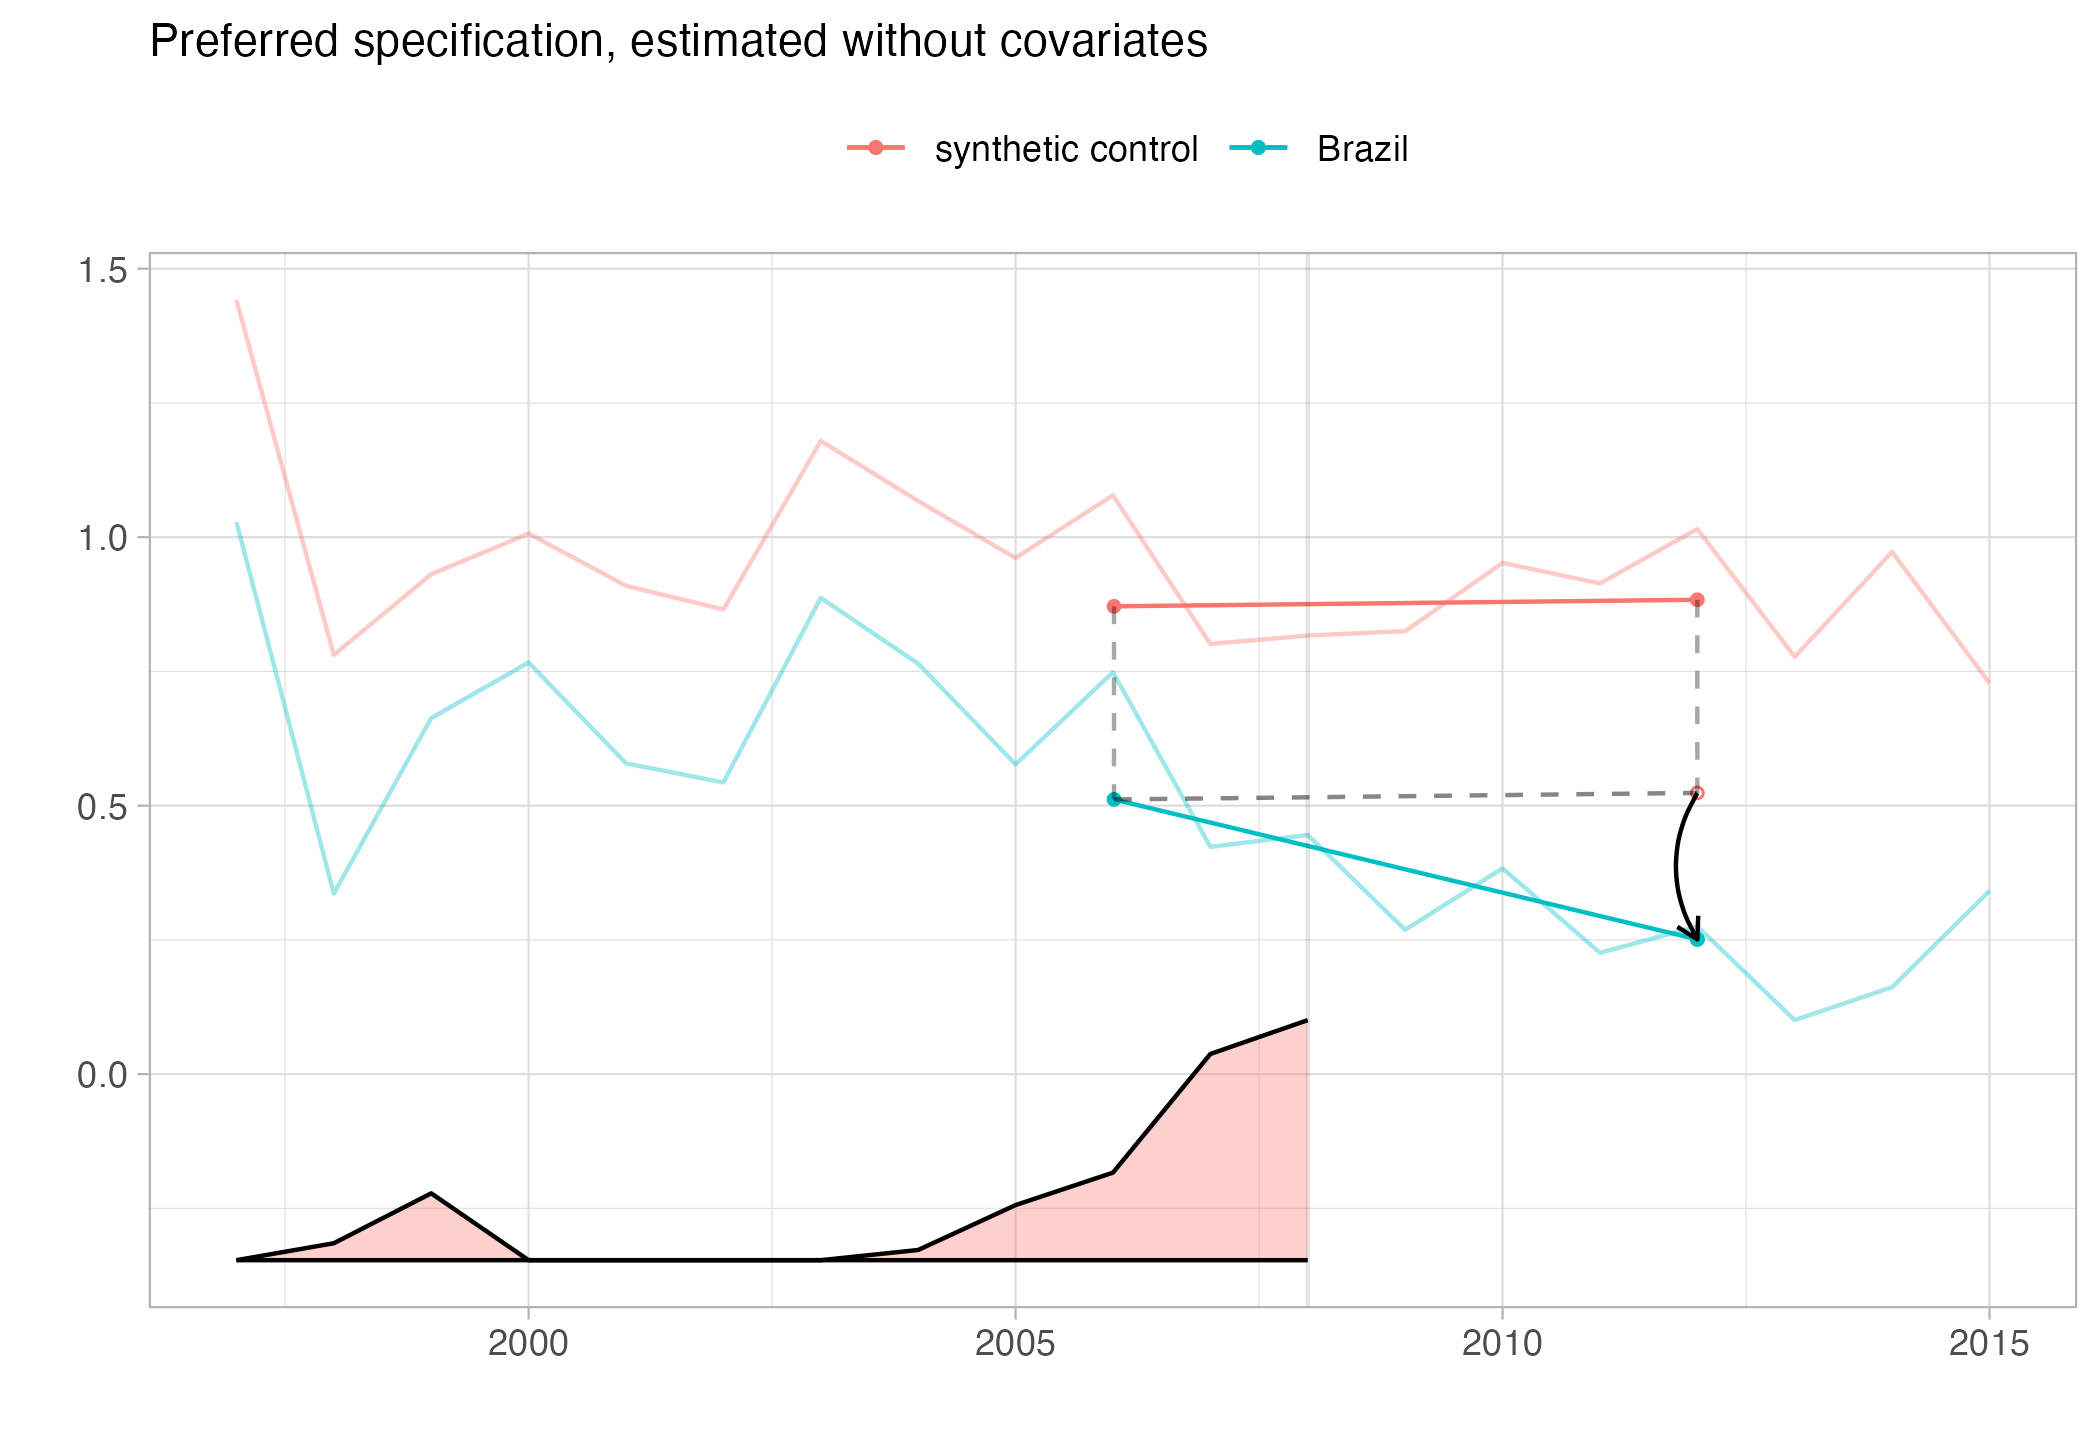
\includegraphics[width=0.95\linewidth]{quality_reports/china_demand_shock_rank_threshold/figure_brazil_sdid_predetermined_core_fit} \caption{Preferred SDiD fit for Brazil and its synthetic comparison, estimated without covariates. Lower values indicate convergence toward China; the post-treatment gap is the average post-2009 reduced-form estimate. Note: Absolute UNGA ideal-point distance to China. SE: placebo-based SE with 20,000 replications; p-values reported in the text and table. Window: 1997-2015 annual Brazil series.}\label{fig:plot-sdid}
\end{figure}

Figure \ref{fig:plot-placebo-distribution} shows the placebo-in-space distribution behind that inference. Brazil sits in the left tail of the estimates obtained by reassigning treatment to each donor in turn.

\begin{figure}
\centering
\pandocbounded{
\includegraphics[keepaspectratio,alt={\label{fig:plot-placebo-distribution}Distribution of placebo-in-space estimates across the 95 donor assignments, with Brazil marked. Brazil's estimate is the 3rd most negative of 96 assignments (directional p = 0.031); the two-sided absolute rank is 7/96 (p = 0.073). Negative values indicate convergence toward China. Note: Estimated post-2009 gap in absolute UNGA ideal-point distance to China. Window: 1997-2015 annual SDiD panel.}]{paper_v4_files/figure-latex/plot-placebo-distribution-1.pdf}}
\caption{\label{fig:plot-placebo-distribution}Distribution of placebo-in-space estimates across the 95 donor assignments, with Brazil marked. Brazil's estimate is the 3rd most negative of 96 assignments (directional p = 0.031); the two-sided absolute rank is 7/96 (p = 0.073). Negative values indicate convergence toward China. Note: Estimated post-2009 gap in absolute UNGA ideal-point distance to China. Window: 1997-2015 annual SDiD panel.}
\end{figure}

Table \ref{tab:brazil-sdid-diagnostic-summary} summarizes the diagnostic package behind the preferred Brazil SDiD estimate. The top five donors are Georgia 3.1\%, Singapore 2.9\%, Chad 2.8\%, Guatemala 2.7\%, Paraguay 2.7\%, and the complete donor pool, along with pre-treatment time weights and sensitivity diagnostics based on donor-deletion and window tests, appears in Appendix Tables \ref{tab:sdid-unit-weights-complete}, \ref{tab:sdid-time-weights}, \ref{tab:sdid-donor-sensitivity}, and \ref{tab:sdid-window-sensitivity}.

One may wonder whether a synthetic control built from donors all over the world is a good counterfactual for Brazil. Column (5) of Table \ref{tab:outcome-robustness-table} re-estimates the preferred specification on a donor pool restricted to Latin American countries. The estimated effect is larger in absolute terms, -0.326 against -0.273 in the global pool, and Brazil is the 2nd most negative of 20 assignments in the directional placebo comparison (p = 0.100). The regional pool is small, which limits what either inference convention can show: with 20 units the rank test cannot fall below 0.050 however extreme Brazil is, and the placebo standard error rises from 0.131 to 0.207, so the normal-approximation interval includes zero. Figure \ref{fig:plot-latam} reports the regional fit.

\begin{table}[H]
\centering
\caption{\label{tab:brazil-sdid-diagnostic-summary}Compact diagnostic summary for the Brazil SDiD estimate.}
\centering
\fontsize{9}{11}\selectfont
\begin{threeparttable}
\begin{tabular}[t]{>{\raggedright\arraybackslash}p{3.3cm}>{\raggedright\arraybackslash}p{11.0cm}}
\toprule
\textbf{Diagnostic} & \textbf{Result}\\
\midrule
\textbf{Weights} & 95 donors; largest weight = 3.1\%; top five = 14.4\% of total weight. Highest time weights: 2008 35.2\%, 2007 30.2\%, 2006 12.8\%, 1999 9.8\%.\\
\cmidrule{1-2}
\textbf{Fit} & Intercept-adjusted pre-treatment RMSPE = 0.058; post/pre adjusted RMSPE ratio = 5.544; Brazil pre-treatment outcome mean = 0.647.\\
\cmidrule{1-2}
\textbf{Placebo inference} & Directional rank = 3/96 (p = 0.031); bilateral absolute rank = 7/96 (p = 0.073).\\
\cmidrule{1-2}
\textbf{Donor sensitivity} & Largest leave-one-donor change = 3.6\%; top-ten donor deletion estimate = -0.268. High-weight donors with China in the post-2009 top two carry 10.2\% of total weight.\\
\cmidrule{1-2}
\textbf{Windows and timing} & 7/7 window estimates are negative (range -0.320 to -0.256). China rank-2 timing estimate in 2004 = -0.109; actual 2009 timing estimate = -0.273.\\
\bottomrule
\end{tabular}
\begin{tablenotes}
\item \textit{Note: } 
\item The preferred fit and its placebo SE come from the targets pipeline; a separate diagnostic script regenerates the tables from those targets. RMSPE diagnostics are intercept-adjusted. Negative estimates mean reduced absolute UNGA ideal-point distance to China. Donor-deletion, timing, and alternative-window rows are point-estimate diagnostics unless inference is explicitly reported.
\end{tablenotes}
\end{threeparttable}
\end{table}

Table \ref{tab:outcome-robustness-table} reports the preferred Brazil SDiD estimate alongside three comparisons. Column (1) uses no covariates and is preferred because it avoids conditioning the counterfactual on variables observed after 2009. Column (2) restores the full contemporaneous covariate matrix; column (3) removes institutional variables but retains the other contemporaneous measures; and column (4) changes the donor pool to Latin America using the contemporaneous matrix. All four estimates are negative, but columns (2)--(4) are sensitivity checks rather than alternative candidates for the main specification.

\begin{table}[H]
\centering
\caption{\label{tab:outcome-robustness-table}Brazil SDiD estimates across main and robustness specifications.}
\centering
\resizebox{\ifdim\width>\linewidth\linewidth\else\width\fi}{!}{
\fontsize{9}{11}\selectfont
\begin{threeparttable}
\begin{tabular}[t]{lccccc}
\toprule
  & (1) Preferred: no covariates & (2) Current covariates & (3) No institutions & (4) Latin America, covariates & (5) Latin America, none\\
\midrule
ATT & -0.273** & -0.268* & -0.269* & -0.408** & -0.326\\
 & (0.131) & (0.143) & (0.143) & (0.207) & (0.207)\\
\textit{Covariates:} &  &  &  &  & \\
Trade share China &  & $\checkmark$ & $\checkmark$ & $\checkmark$ & \\
Trade share US &  & $\checkmark$ & $\checkmark$ & $\checkmark$ & \\
\addlinespace
Power index (GPI) &  & $\checkmark$ & $\checkmark$ & $\checkmark$ & \\
Power gap to US &  & $\checkmark$ & $\checkmark$ & $\checkmark$ & \\
Per-capita income &  & $\checkmark$ & $\checkmark$ & $\checkmark$ & \\
Exchange rate &  & $\checkmark$ & $\checkmark$ & $\checkmark$ & \\
Geographic distance to US &  & $\checkmark$ & $\checkmark$ & $\checkmark$ & \\
\addlinespace
HoG left ideology &  & $\checkmark$ & $\checkmark$ & $\checkmark$ & \\
Current account (\% GDP) &  & $\checkmark$ & $\checkmark$ & $\checkmark$ & \\
Gov. deficit (\% GDP) &  & $\checkmark$ & $\checkmark$ & $\checkmark$ & \\
Parliamentary system &  & $\checkmark$ &  & $\checkmark$ & \\
Military executive &  & $\checkmark$ &  & $\checkmark$ & \\
\addlinespace
US trade agreement &  & $\checkmark$ &  & $\checkmark$ & \\
Country-years & 1,824 & 1,824 & 1,824 & 380 & 380\\
Donor countries & 95 & 95 & 95 & 19 & 19\\
Donor pool & Global & Global & Global & Latin America & Latin America\\
Time window & 1997-2015 & 1997-2015 & 1997-2015 & 1997-2015 & 1997-2015\\
\bottomrule
\end{tabular}
\begin{tablenotes}
\item \textit{Note: } 
\item The outcome is absolute UNGA ideal-point distance to China; ATT is the estimated average causal effect on Brazil after 2009, so negative values mean convergence. ATTs are reported with three decimals. Placebo-based SEs are in parentheses (20,000 replications for the preferred column; 5,000 for the comparison columns). Stars use two-sided normal-approximation p-values based on placebo SEs: * p < 0.10; ** p < 0.05; *** p < 0.01. Checkmarks show included covariate groups. Donor counts exclude Brazil. Column (1) uses no covariates, so its covariate cells are left blank. Columns (2)-(4) use contemporaneous covariates and are comparisons. Column (5) applies the preferred no-covariate specification to the Latin American donor pool, so it is the column comparable with (1); its directional placebo rank is 2/20 (p = 0.100), against a floor of 0.050 imposed by the size of the regional pool. For column (1), the directional rank is 3/96 (p = 0.031) and the bilateral absolute rank is 7/96 (p = 0.073).
\end{tablenotes}
\end{threeparttable}}
\end{table}

The rank interpretation requires more than showing that trade with China was increasing. Brazil's exports to China grew before 2009, including years in which China rose in the export hierarchy but did not become number one. Table \ref{tab:table-placebo} therefore reports outcome-path timing falsifications without covariates: using no covariates prevents variables measured after the early pseudo-onsets from entering those comparisons. The 2003, 2004, and 2005 estimates are smaller than the 2009 rank-one estimate; 2004 is especially useful because China first reaches rank \#2 but is still not Brazil's largest export destination. The 2012 row probes a later break after China had already become the top destination. These are point-estimate diagnostics rather than additional tests with separately recomputed placebo inference.

The same timing logic addresses the main Brazilian political confounder. President Lula da Silva took office in 2003 and pursued a more explicit South-South foreign-policy agenda, a shift emphasized in work on Brazilian autonomy, presidential foreign policy, and international engagement (\citeproc{ref-neto2011}{Neto 2011}; \citeproc{ref-mouron_urdinez2014}{Mourón and Urdinez 2014}; \citeproc{ref-neto_malamud2015}{Neto and Malamud 2015}; \citeproc{ref-rodrigues2019measuring}{P. Rodrigues, Urdinez, and De Oliveira 2019}; \citeproc{ref-schenoniMythsMultipolaritySources2022}{Luis L. Schenoni et al. 2022}). If that ideological shift were sufficient to explain Brazil-China UNGA convergence, the pseudo-treatment years in 2003 or 2005 should already show comparable movement. They do not. The cross-country panel also estimates the rank-threshold pattern across countries with different political systems and leadership profiles, which reduces the concern that the Brazil estimate is only a Lula-period artifact.

A remaining concern is that 2009 bundled the Brazilian rank reversal with other contemporaneous shocks, including the global financial crisis, the BRICS/G20 moment, and the commodity cycle. Table \ref{tab:china-demand-sdid-diagnostics} uses a measure built from external goods exports only to address this critique. Brazil's 2004--2008 primary-goods share is 29.04 percent, composed of 11.25 percent Agriculture and 17.79 percent Mining and Energy. The preferred ATT is -0.273; adding primary composition and its 2008--2009 interaction yields -0.285. Composition, decomposition, global-price, and prior-China-exposure specifications remain in a narrow negative range. The 2008--2009 interactions are robustness or mechanism diagnostics, not alternative total-effect estimates, because 2009 is the first treated year and the interaction may absorb part of the mechanism. Stability across these measures does not isolate the rank cue experimentally from every 2009 political shock, but it reduces the narrower concern that the preferred estimate is an artifact of post-treatment controls or omitted pre-2009 commodity composition.

The cross-country panel below is a broader scope check, not the main answer to the Brazil-specific demand-shock critique. Brazil is included in the goods-only cross-country sample, but the panel aligns countries by their own China-top goods-export entry years. A Brazil-specific 2009 confounder cannot mechanically generate an average event-time effect across countries treated in different calendar years. For such an explanation to account for both the Brazil estimate and the cross-country result, the omitted force would need to coincide with durable China-top entry across countries, affect UNGA distance to China in the same direction, and remain outside the latent factors captured by the interactive fixed-effects specification. In sensitivity-analysis terms, it would need enough residual association with both treatment timing and the outcome to overturn estimates that are stable across the Brazil timing tests, donor-pool checks, and the cross-country duration and risk-set checks (\citeproc{ref-cinelli_hazlett2020}{Cinelli and Hazlett 2020}; \citeproc{ref-oster2019}{Oster 2019}).

\begin{table}[H]
\centering
\caption{\label{tab:table-placebo}Brazil SDiD rank-versus-volume timing diagnostics without covariates.}
\centering
\resizebox{\ifdim\width>\linewidth\linewidth\else\width\fi}{!}{
\fontsize{8}{10}\selectfont
\begin{threeparttable}
\begin{tabular}[t]{clccccl}
\toprule
Timing year & Test role & China rank & Export share (\%) & Margin (USD bn) & ATT & Inference\\
\midrule
2003 & Growth/lower-rank promotion & 3 & 6.7 & -12.9 & -0.064 & Point estimate only; no covariates\\
2004 & China rank-2 threshold & 2 & 7.4 & -14.2 & -0.109 & Point estimate only; no covariates\\
2005 & Rapid growth without rank 1 & 3 & 7.2 & -16.7 & -0.099 & Point estimate only; no covariates\\
2009 & Actual rank-1 reversal & 1 & 15.1 & 4.1 & -0.273 & Point estimate only; no covariates\\
2012 & Later-break falsification & 1 & 18.8 & 14.9 & -0.100 & Point estimate only; no covariates\\
\bottomrule
\end{tabular}
\begin{tablenotes}
\item \textit{Note: } 
\item Outcome is absolute UNGA ideal-point distance to China; ATT is the estimated causal effect on Brazil after the nominal onset, so negative values mean convergence; export margins are current USD billions. Window: 2003-2005 timing tests end in 2008; 2012 is a later-break falsification using data through 2016. All rows are no-covariate point-estimate diagnostics. The preferred 2009 estimate and its inference are reported separately in the main specification.
\end{tablenotes}
\end{threeparttable}}
\end{table}

\begin{table}[H]
\centering
\caption{\label{tab:china-demand-sdid-diagnostics}Brazil SDiD estimates under corrected predetermined commodity and China-demand diagnostics.}
\centering
\fontsize{9}{11}\selectfont
\begin{threeparttable}
\begin{tabular}[t]{lcccc}
\toprule
Specification & ATT & Placebo SE & Normal p & Rank p (dir./bilat.)\\
\midrule
Current covariates & -0.268 & 0.143 & 0.061 & Not computed\\
Preferred: no covariates & -0.273 & 0.131 & 0.037 & 0.031 / 0.073\\
Primary share x 2008-2009 & -0.285 & 0.129 & 0.027 & 0.031 / 0.073\\
Agriculture/mining x 2008-2009 & -0.284 & 0.128 & 0.026 & Not computed\\
Price exposure x 2008-2009 & -0.277 & 0.130 & 0.034 & Not computed\\
\addlinespace
Prior China share x 2008-2009 & -0.284 & 0.130 & 0.029 & Not computed\\
\bottomrule
\end{tabular}
\begin{tablenotes}
\item \textit{Note: } 
\item Outcome is absolute UNGA ideal-point distance to China; ATT is the estimated average causal effect on Brazil after 2009, so negative values mean convergence. SE: synthdid placebo SE with 5,000 replications. Window: 1997-2015 annual SDiD panel. All rows keep the binary 2009 China number-one treatment onset. Comparison rows use 5,000-replication placebo SEs with a common permutation seed; the preferred row reuses the pipeline standard error (20,000 replications). The preferred row uses no covariates; the current-covariates row is a comparison. Primary-goods measures use external goods exports only. The 2008-2009 interactions include the first treated year and are mechanism robustness checks, not preferred total-effect specifications. Rank inference was computed for the preferred specification and the primary-share x 2008-2009 interaction; 'Not computed' does not denote a failed test.
\end{tablenotes}
\end{threeparttable}
\end{table}

\subsection{Issue-Area Evidence: Where Did Convergence Occur?}\label{issue-area-evidence-where-did-convergence-occur}

The aggregate ideal-point estimate raises a substantive question: in what kinds of votes did Brazil move closer to China? Resolution-level diagnostics suggest that the post-2009 convergence was selective rather than uniform. In several issue areas Brazil and China already voted together at high rates before treatment, leaving little room for additional convergence. The more informative domain is human rights, where pre-treatment agreement was lower and where movement toward China carried greater reputational costs for Brazil, given the domestic and international implications of Brazil's human-rights foreign policy (\citeproc{ref-milani2015humanrights}{Milani 2015}). In that domain, Brazil-China identical voting increased by 7.5 percentage points after 2009. This pattern is consistent with the proposed mechanism: the trade-rank cue made China's relationship politically usable, allowing policymakers to justify selective convergence in a visible multilateral arena where Brazil had previously maintained more distance.

This descriptive increase does not by itself establish China-specific alignment, because annual issue-area shares can reflect agenda composition and do not compare Brazil with donor countries. I therefore add a more restrictive vote-level diagnostic. In country-resolution regressions with country and resolution fixed effects, restricted to human-rights votes where China and the United States cast different votes, Brazil moves closer to China after 2009 relative to the donor pool. The Brazil-by-post-2009 coefficient is -0.357 for distance to China minus distance to the United States (model-based SE = 0.021), and -0.414 when the sample is restricted to strong yes/no China-US disagreements (model-based SE = 0.023). The corresponding non-human-rights estimate is smaller (-0.131, model-based SE = 0.012), and a triple-difference specification estimates an additional human-rights increment of -0.264 (model-based SE = 0.055). Restricting attention to a single issue domain opens a design that ideal points computed over all votes cannot support: a triple difference. Ideal points compress every resolution in a session into one score, leaving no contrast between issue domains to exploit, whereas vote-level data preserve it. The third difference is therefore across domains within the same country and year, comparing Brazil with the donor pool, before and after 2009, in human-rights votes relative to every other vote. Brazil remains the only treated country; the design adds a dimension of comparison, not treated units. Identification here asks for more than parallel trends between treated and control units: whatever bias a non-parallel trend introduces must be the same in the two issue domains, so that it cancels in the third difference (\citeproc{ref-olden_moen2022}{Olden and Møen 2022}). Because this evidence corroborates the main result and locates part of the mechanism rather than carrying the causal claim on its own, that requirement is less demanding than in the main design. Appendix Figure \ref{fig:plot-ddd-pretrends} shows that Brazil's distance from the donor pool moves in parallel across the two domains before 2009 and separates afterwards. Because Brazil is the single treated country in this diagnostic, I use country placebos as the main inferential benchmark: Brazil ranks 6 out of 95 units in the China-specific direction (directional p = 0.063; strict donor-only p = 0.053). These diagnostics support a narrower interpretation: the post-2009 movement is strongest in human-rights votes where China and the United States diverged, rather than uniformly across the UNGA agenda.

\begin{table}[H]
\centering
\caption{\label{tab:issue-area-prepost-table}Brazil-China identical UNGA votes by issue area, before and after 2009.}
\centering
\resizebox{\ifdim\width>\linewidth\linewidth\else\width\fi}{!}{
\fontsize{8}{10}\selectfont
\begin{threeparttable}
\begin{tabular}[t]{lrrrl}
\toprule
Issue area & Pre-2009 identical vote share & Post-2009 identical vote share & Change & Interpretation\\
\midrule
Human rights & 69.6 & 77.1 & 7.5 & Politically costly convergence; mechanism-informative\\
Arms/disarmament/nuclear & 83.0 & 84.3 & 1.2 & Diagnostic evidence\\
Economic development & 92.9 & 90.0 & -2.9 & Diagnostic evidence\\
Decolonization & 94.1 & 98.1 & 4.0 & Diagnostic evidence\\
Palestine/Middle East & 100.0 & 100.0 & 0.0 & High baseline agreement; limited room to move\\
\addlinespace
Other / uncoded & 73.4 & 83.1 & 9.7 & Heterogeneous residual category\\
\bottomrule
\end{tabular}
\begin{tablenotes}
\item \textit{Note: } 
\item Percentage of roll-call resolutions with identical Brazil-China votes. Window: 2005-2008 versus 2009-2012; multi-coded resolutions enter each issue family. Rows are label-specific diagnostics, not a mutually exclusive decomposition of the aggregate convergence pattern.
\end{tablenotes}
\end{threeparttable}}
\end{table}

Figure \ref{fig:plot-brazil-china-unvotes-issue-year} disaggregates the same diagnostic by year and substantive issue family. Because several areas already had high Brazil-China vote similarity before 2009, the figure describes where additional convergence was possible.

\begin{figure}
\centering
\pandocbounded{
\includegraphics[keepaspectratio,alt={\label{fig:plot-brazil-china-unvotes-issue-year}Brazil-China identical UNGA votes by issue area, 2005-2012. Points report annual shares; the vertical line marks 2009. The clearest pattern expected by the mechanism is selective convergence in human rights. Note: Percentage of roll-call resolutions with identical Brazil-China votes. Window: 2005-2012 annual series; multi-coded resolutions enter each issue family.}]{paper_v4_files/figure-latex/plot-brazil-china-unvotes-issue-year-1.pdf}}
\caption{\label{fig:plot-brazil-china-unvotes-issue-year}Brazil-China identical UNGA votes by issue area, 2005-2012. Points report annual shares; the vertical line marks 2009. The clearest pattern expected by the mechanism is selective convergence in human rights. Note: Percentage of roll-call resolutions with identical Brazil-China votes. Window: 2005-2012 annual series; multi-coded resolutions enter each issue family.}
\end{figure}

The strongest support comes from human-rights resolutions in which China and the United States diverged, where Brazil moves closer to China relative to comparable donor countries after 2009. A DDD comparison shows that the human-rights shift is larger than the analogous non-human-rights shift. Country placebos counsel against language implying that Brazil is unique. The Brazil evidence therefore supports a cautious claim of selective UNGA adjustment toward China in politically visible domains, rather than a claim that the issue-area table alone proves selective convergence.

\section{Brazilian media salience}\label{brazilian-media-salience}

To assess whether the rank reversal became publicly salient, I examine coverage of China in Folha de S.Paulo, Brazil's widest-circulation newspaper (\citeproc{ref-folha2016}{Folha de S.Paulo 2016}), from 2000 to 2014. Salience matters because the rank-threshold argument requires the top-rank cue to become politically usable. A change in export hierarchy can shape elite and public attention when it appears in a prominent national newspaper as a simple signal of China's commercial importance, consistent with work on media, agenda setting, and foreign policy (\citeproc{ref-soroka2003}{Soroka 2003}; \citeproc{ref-baum_potter2008}{Baum and Potter 2008}; \citeproc{ref-walgraveContingencyMassMedias2006}{Walgrave and Van Aelst 2006}).

Headlines are the appropriate unit for this diagnostic because the mechanism is public attention and categorical labeling. This follows corpus-assisted media studies that use headlines because they are tractable in large archives and operate as attention-directing cues (\citeproc{ref-zhang_yu2024_chinese_dream}{Zhang and Yu 2024}). The relevant question is whether Folha increasingly foregrounded China as a trade relationship after the rank reversal. Headlines are the most visible textual cue in the archive, they are the part of coverage most likely to be scanned by broad audiences, and they are where newspapers condense complex developments into short public labels such as ``largest trade partner'' or ``record exports.'' Full article texts would be useful for a different exercise -- for example, measuring tone or detailed argumentation -- but the salience claim here is about which China-related themes were made visible at the headline level.

I therefore classify China-related headlines into substantive categories and then collapse them into four analytically relevant groups: China-Brazil trade, China's domestic economy, diplomacy and bilateral relations, and non-economic coverage. The classification uses a fixed label set with examples, and the appendix reports the exact prompt and validation procedure. Figure \ref{fig:plot-media-counterfactual} shows that the post-2009 increase is concentrated in China-Brazil trade coverage rather than in all China-related topics equally. This pattern is consistent with a rank-salience interpretation: coverage concentrates on China's new commercial status in Brazil.

\begin{figure}
\centering
\pandocbounded{
\includegraphics[keepaspectratio,alt={\label{fig:plot-media-counterfactual}Brazilian media salience: disaggregated China headlines in Folha de S.Paulo by category. The sustained post-2009 increase is concentrated in trade-related coverage. Note: Headlines per category per year. Window: 2000-2014 annual series.}]{paper_v4_files/figure-latex/plot-media-counterfactual-1.pdf}}
\caption{\label{fig:plot-media-counterfactual}Brazilian media salience: disaggregated China headlines in Folha de S.Paulo by category. The sustained post-2009 increase is concentrated in trade-related coverage. Note: Headlines per category per year. Window: 2000-2014 annual series.}
\end{figure}

\clearpage

The media evidence documents public availability and official uptake of the attention cue. The status cue became publicly available during the 2009 treatment year, before the full-year trade table was finalized. In early May, contemporary coverage of January--April trade statistics reported a historic shift in Brazil's trade hierarchy: China had become Brazil's largest trading partner and had purchased US\$5.627 billion in Brazilian exports, compared with US\$4.925 billion purchased by the United States (\citeproc{ref-agencia_brasil2009_china_supera}{Agência Brasil 2009}). This real-time visibility matters for the mechanism. The empirical design codes treatment annually because the outcome and comparative trade data are annual, but officials, journalists, and firms encountered the rank cue through contemporaneous monthly and year-to-date statistics. Lula's May 2009 Beijing visit therefore provides evidence of official uptake during the treatment year: the new rank was already available as a public category around which diplomatic priorities could be narrated. Brazilian officials then repeatedly invoked China's new position in Brazil's trade hierarchy when explaining diplomatic prioritization, bilateral upgrading, and institutional follow-up.

In a written interview on the eve of his May 2009 visit to Beijing, President Lula described China as Brazil's leading trading partner and framed the trip as an effort to consolidate cooperation across commerce, technology, and global economic governance (\citeproc{ref-mre_funag_resenha104_2009}{Ministério das Relações Exteriores and Fundação Alexandre de Gusmão 2009, 323}). In Beijing three days later, Lula repeated the rank claim in speeches organized around the Brazil-China Strategic Partnership, trade diversification, investment, presidential diplomacy, and the preparation of the 2010--2014 Joint Action Plan (\citeproc{ref-mre_funag_resenha104_2009}{Ministério das Relações Exteriores and Fundação Alexandre de Gusmão 2009, 115, 121--22}). The cue then persisted in Itamaraty language. When announcing Hu Jintao's 2010 state visit and the signature of the Joint Action Plan, the Ministry of Foreign Affairs again invoked China's 2009 rise to the top of Brazil's trade hierarchy (\citeproc{ref-mre_funag_resenha106_2010}{Ministério das Relações Exteriores and Fundação Alexandre de Gusmão 2010, 356}). Dilma Rousseff and Hu Jintao's 2011 joint communiqué likewise noted that China had become Brazil's principal trading partner in 2009 and embedded that status in an agenda of intensified dialogue over trade, investment, diversification, and implementation of the Joint Action Plan (\citeproc{ref-mre_funag_resenha108_2011}{Ministério das Relações Exteriores and Fundação Alexandre de Gusmão 2011a, 160--61}). Later that year, Foreign Minister Antonio Patriota made the institutional link explicit: in discussing China, he announced a dedicated Itamaraty task force to monitor economic-commercial relations with Brazil's principal trading partner and to propose ways to move the relationship beyond complementarity, toward diversification and higher value-added trade (\citeproc{ref-mre_funag_resenha109_2011}{Ministério das Relações Exteriores and Fundação Alexandre de Gusmão 2011b, 47}).

These statements show that the 2009 status cue was absorbed into official language in ways consistent with justificatory use for diplomatic prioritization and institutional attention. This matches the public mechanism implied by the theory: once China was officially recognized as central in Brazil's economic hierarchy, selective diplomatic accommodation could be presented as pragmatic recognition of national economic interests rather than as ideological concession or opportunistic bandwagoning.

\section{Cross-Country Evidence Beyond Brazil}\label{cross-country-evidence-beyond-brazil}

The cross-country analysis serves two purposes. First, it tests whether durable top-rank goods-export status is followed by movement toward China beyond the Brazilian case. Second, it is an additional robustness check against explanations tied to Brazil's 2009 calendar year, such as the global financial crisis, the BRICS/G20 moment, or the commodity cycle. If durable top-rank trade status matters, countries where China enters and holds the largest goods export-destination position should move closer to China in UNGA ideal-point space when aligned by their own treatment entry. I therefore estimate the same treatment logic in a goods-only status-current panel: treated country-years are those where China is rank 1 among goods export destinations and the China-top period lasts at least five observed years. Never-China-top countries remain controls. Short China-top episodes and post-exit off-status years for treated countries are removed from the main risk set. This analysis evaluates whether the rank-threshold pattern is compatible with evidence beyond the theory-generating case while matching the durable treatment observed in Brazil.

The preferred cross-country specification is the no-covariate IFE model on the goods-only restricted risk set. The estimate is -0.101 ideal-point units (bootstrap SE = 0.039, 95 percent CI {[}-0.177, -0.024{]}, p = 0.010). It corresponds to about 14.0 percent of the pre-treatment mean distance to China, or 0.124 standard deviations of the outcome. The estimate is in the theoretically expected negative direction and statistically distinguishable from zero at the 5 percent level. The clean single-entry robustness estimate is -0.122 (p = 0.003). The switching-allowed estimate is smaller, -0.037 (p = 0.214), which is consistent with attenuation when short China-top periods and post-exit off-status years are allowed into the comparison structure. The cross-country evidence is smaller than the Brazil SDiD effect, consistent with Brazil being a most-likely case in which China displaced the United States and the rank reversal was publicly salient. The direction is the same: durable China-top goods-export status is associated with reduced UNGA distance to China beyond the Brazilian case. Appendix Tables \ref{tab:cross-country-duration-table} and \ref{tab:cross-country-audit-table} report duration-threshold robustness and sample-coding audits.

\begin{table}[H]
\centering
\caption{\label{tab:cross-country-table}Cross-country IFE estimates for durable China top goods export-destination status.}
\centering
\resizebox{\ifdim\width>\linewidth\linewidth\else\width\fi}{!}{
\fontsize{8}{10}\selectfont
\begin{threeparttable}
\begin{tabular}[t]{llcccccccc}
\toprule
Model & Estimator & ATT & SE & 95\% CI & p-value & Units (T/C) & Treated periods & Panel window & r*\\
\midrule
Status-current, restricted risk set & IFE & -0.101 & 0.039 & {}[-0.177, -0.024] & 0.010 & 35/126 & 440 & 1990--2022 & 2\\
Clean single-entry robustness & IFE & -0.122 & 0.041 & {}[-0.202, -0.042] & 0.003 & 25/126 & 329 & 1990--2022 & 2\\
Status-current, switching allowed & IFE & -0.037 & 0.030 & {}[-0.096, 0.022] & 0.214 & 24/89 & 297 & 1990--2022 & 1\\
\bottomrule
\end{tabular}
\begin{tablenotes}
\item \textit{Note: } 
\item ATT in absolute UNGA ideal-point distance to China; lower values indicate convergence toward China. SE: bootstrap with 10,000 replications. Window: 1990--2022 goods-only cross-country panel. Goods-only ranks are computed from ITPD-E Agriculture, Mining and Energy, and Manufacturing sectors; Services are excluded before ranks are constructed. Units (T/C) = treated/control units. For IFE rows, r* is the number of latent factors selected by cross-validation over r = 0:3. The restricted risk-set row is the main cross-country estimate. The clean single-entry row excludes treated countries with multiple China-top periods. The switching-allowed row is a status-current robustness check that keeps a balanced panel and changes the comparison structure.
\end{tablenotes}
\end{threeparttable}}
\end{table}

Figure \ref{fig:cross-country-dynamic} shows the entry-aligned dynamic pattern for the main goods-only restricted-risk-set IFE specification. The pre-entry estimates are diagnostics for model fit, and the post-entry path indicates whether the panel pattern is consistent with the Brazil result. Event-time tails with few treated units are descriptive; the average ATT and the duration-threshold table are the better-supported cross-country summaries.

\begin{figure}
\centering
\pandocbounded{\includegraphics[keepaspectratio,alt={\label{fig:cross-country-dynamic}Entry-aligned dynamic effects from the main goods-only cross-country IFE model. Negative estimates indicate reduced UNGA distance to China after entry into durable status as the top goods-export destination. Event-time tails with few treated units should be read descriptively. Note: Effect on absolute UNGA ideal-point distance to China. SE: bootstrap confidence intervals. Window: 1990--2022 goods-only panel.}]{paper_v4_files/figure-latex/cross-country-dynamic-1.pdf}}
\caption{\label{fig:cross-country-dynamic}Entry-aligned dynamic effects from the main goods-only cross-country IFE model. Negative estimates indicate reduced UNGA distance to China after entry into durable status as the top goods-export destination. Event-time tails with few treated units should be read descriptively. Note: Effect on absolute UNGA ideal-point distance to China. SE: bootstrap confidence intervals. Window: 1990--2022 goods-only panel.}
\end{figure}

The two designs test nested implications of the argument. Brazil is the high-salience case: China displaced the United States, the hegemonic benchmark, and the attention mechanism can be observed directly in media and official discourse. The cross-country panel tests a broader scope implication: whether durable status as the top goods-export destination is followed by movement toward China when local salience is less directly observable. The panel estimate should therefore be interpreted as scope evidence rather than as a substitute for the Brazilian mechanism test.

The cross-country treatment is durable status-current China-top goods-export-destination status, the exposure rule implied by the theory's durability condition. The corresponding estimand is the ATT on absolute UNGA ideal-point distance to China for country-years in qualifying China-top periods.

\section{Conclusion}\label{conclusion}

The evidence supports a rank-threshold account of UNGA voting convergence toward China. In Brazil, China's 2009 move into the top export-destination position coincided with a publicly visible status cue. In the preferred SDiD specification, the estimated effect is a reduction of 0.272 ideal-point units in Brazil's distance to China relative to its synthetic counterfactual. Conventional inference and the theory-aligned directional placebo comparison support a negative effect, while the conservative two-sided placebo comparison is less decisive. The issue-area and vote-level evidence suggest that this convergence was selective rather than mechanical: the strongest additional support comes from human-rights resolutions where China and the United States diverged, and the human-rights shift is larger than the analogous non-human-rights shift. The media evidence shows that the rank cue was publicly available and politically usable: China's new commercial status became visible in Folha headlines and official discourse. Cross-country estimates from the goods-only IFE model then show a compatible directional pattern beyond Brazil. The mechanism is measured most directly in the Brazilian case, and the panel evidence extends the argument beyond the theory-generating case: durable top-rank goods-export milestones can matter for multilateral alignment.

The paper therefore shifts attention from trade volume alone to the political meaning of trade hierarchies. Continuous exposure matters, but actors also respond to categorical milestones: becoming first, displacing a hegemonic benchmark, and making an economic relationship publicly legible. These thresholds can create opportunities for selective diplomatic adjustment even when the underlying commercial relationship has been growing for years.

Future research can extend the design in three directions. First, cross-country media data would allow the salience step to be tested beyond Brazil. Second, qualitative work on policymakers and business actors could identify how the rank cue entered diplomatic deliberation. Third, similar rank-threshold designs could be applied to investment, aid, lending, or other economic ties where categorical milestones may become politically usable.

\clearpage

\section*{References}\label{references}
\addcontentsline{toc}{section}{References}

\protect\phantomsection\label{refs}
\begin{CSLReferences}{1}{0}
\bibitem[\citeproctext]{ref-agencia_brasil2009_china_supera}
Agência Brasil. 2009. {``China supera Estados Unidos e torna-se maior parceiro comercial do Brasil.''} \emph{Agência Brasil}, May. \url{https://memoria.ebc.com.br/agenciabrasil/noticia/2009-05-04/china-supera-estados-unidos-e-torna-se-maior-parceiro-comercial-do-brasil}.

\bibitem[\citeproctext]{ref-arkhangelsky_etal2021}
Arkhangelsky, Dmitry, Susan Athey, David A. Hirshberg, Guido W. Imbens, and Stefan Wager. 2021. {``Synthetic {Difference-in-Differences}.''} \emph{American Economic Review} 111 (12): 4088--118. \url{https://doi.org/10.1257/aer.20190159}.

\bibitem[\citeproctext]{ref-bailey_etal2017}
Bailey, Michael A, Anton Strezhnev, and Erik Voeten. 2017. {``Estimating Dynamic State Preferences from {United Nations} Voting Data.''} \emph{Journal of Conflict Resolution} 61 (2): 430--56.

\bibitem[\citeproctext]{ref-baum_potter2008}
Baum, Matthew A., and Philip B. K. Potter. 2008. {``The {Relationships Between Mass Media}, {Public Opinion}, and {Foreign Policy}: {Toward} a {Theoretical Synthesis}.''} \emph{Annual Review of Political Science} 11: 39--65. \url{https://doi.org/10.1146/annurev.polisci.11.060406.214132}.

\bibitem[\citeproctext]{ref-bbc2021}
BBC News. 2021. {``China Overtakes {US} as {EU}'s Biggest Trading Partner.''} \url{https://www.bbc.com/news/business-56093378}.

\bibitem[\citeproctext]{ref-borchert_etal2021}
Borchert, Ingo, Mario Larch, Serge Shikher, and Yoto V Yotov. 2021. {``The International Trade and Production Database for Estimation ({ITPD-E}).''} \emph{International Economics} 166: 140--66.

\bibitem[\citeproctext]{ref-bordalo_etal2022}
Bordalo, Pedro, Nicola Gennaioli, and Andrei Shleifer. 2022. {``Salience.''} \emph{Annual Review of Economics} 14: 521--44. \url{https://doi.org/10.1146/annurev-economics-051520-011616}.

\bibitem[\citeproctext]{ref-brun_covarrubias2024}
Brun, Élodie, and Ana Covarrubias. 2024. {``The Meanings of Autonomy: {Brazilian} and Mexican Reactions to Tensions Between China and the United States.''} \emph{Revista Brasileira de Pol{ı́}tica Internacional} 67 (2): e025.

\bibitem[\citeproctext]{ref-cinelli_hazlett2020}
Cinelli, Carlos, and Chad Hazlett. 2020. {``Making Sense of Sensitivity: Extending Omitted Variable Bias.''} \emph{Journal of the Royal Statistical Society: Series B (Statistical Methodology)} 82 (1): 39--67. \url{https://doi.org/10.1111/rssb.12348}.

\bibitem[\citeproctext]{ref-conlon2023}
Conlon, John J. 2025. {``Attention, {Information}, and {Persuasion}.''} Working paper. Carnegie Mellon University. \url{https://johnjconlon17.github.io/website/conlon_attention_persuasion.pdf}.

\bibitem[\citeproctext]{ref-coutinho_rodriguez2024}
Coutinho, Yuri Bravo, and Júlio César Cossio Rodriguez. 2024. {``Chinese {Double Effect} on {Brazilian Foreign Policy} (2003-2018).''} \emph{Contexto Internacional} 46 (2): e20230014. \url{https://doi.org/10.1590/s0102-8529.20244602e20230014}.

\bibitem[\citeproctext]{ref-davis_pratt2021}
Davis, Christina L., and Tyler Pratt. 2021. {``The Forces of Attraction: How Security Interests Shape Membership in Economic Institutions.''} \emph{The Review of International Organizations} 16 (4): 903--29. \url{https://doi.org/10.1007/s11558-020-09395-w}.

\bibitem[\citeproctext]{ref-deng2008_status}
Deng, Yong. 2008. \emph{China's Struggle for Status: The Realignment of International Relations}. New York: Cambridge University Press.

\bibitem[\citeproctext]{ref-dreher_jensen2013}
Dreher, Axel, and Nathan M. Jensen. 2013. {``Country or Leader? {Political} Change and {UN General Assembly} Voting.''} \emph{European Journal of Political Economy} 29: 183--96. \url{https://doi.org/10.1016/j.ejpoleco.2012.10.001}.

\bibitem[\citeproctext]{ref-duque_2018}
Duque, Marina G. 2018. {``Recognizing {International Status}: {A Relational Approach}.''} \emph{International Studies Quarterly} 62 (3): 577--92. \url{https://doi.org/10.1093/isq/sqy001}.

\bibitem[\citeproctext]{ref-enke2024}
Enke, Benjamin. 2024. {``The Cognitive Turn in Behavioral Economics.''} Working paper. {Harvard University and National Bureau of Economic Research}. \url{https://benjamin-enke.com/pdf/Cognitive_turn.pdf}.

\bibitem[\citeproctext]{ref-fjelstul_etal2026}
Fjelstul, Joshua, Simon Hug, and Christopher Kilby. 2026. {``Decision-Making in the {United Nations General Assembly}: A Comprehensive Database of Resolution-Related Decisions.''} \emph{The Review of International Organizations} 21: 447--64. \url{https://doi.org/10.1007/s11558-024-09580-1}.

\bibitem[\citeproctext]{ref-flores-macias_kreps2013}
Flores-Macías, Gustavo A., and Sarah E. Kreps. 2013. {``The {Foreign Policy Consequences} of {Trade}: {China}'s {Commercial Relations} with {Africa} and {Latin America}, 1992--2006.''} \emph{The Journal of Politics} 75 (2): 357--71. \url{https://doi.org/10.1017/S0022381613000066}.

\bibitem[\citeproctext]{ref-folha2016}
Folha de S.Paulo. 2016. {``{Alcance total dos jornais}.''} https://arte.folha.uol.com.br/graficos/QcVNh/.

\bibitem[\citeproctext]{ref-garcia_herrero_etal2024}
Garcia-Herrero, Alicia, Thibault Storella, and Pekka Weil. 2024. {``China's Influence at the {United Nations}: Words and Deeds.''} Working Paper 19/2024. Bruegel.

\bibitem[\citeproctext]{ref-gotz_2021}
Götz, Elias. 2021. {``Status {Matters} in {World Politics}.''} \emph{International Studies Review} 23 (1): 228--47. \url{https://doi.org/10.1093/isr/viaa046}.

\bibitem[\citeproctext]{ref-gowa1995}
Gowa, Joanne. 1995. \emph{Allies, Adversaries, and International Trade}. Princeton University Press.

\bibitem[\citeproctext]{ref-graeber_etal2025}
Graeber, Thomas, Christopher Roth, and Marco Sammon. 2025. {``Coarse Categories in a Complex World.''} CESifo Working Paper 12032. {CESifo}. \url{https://doi.org/10.2139/ssrn.5366458}.

\bibitem[\citeproctext]{ref-guilhon2014}
Guilhon-Albuquerque, José-Augusto. 2014. {``Brazil, {China}, {US}: A Triangular Relation?''} \emph{Revista Brasileira de Pol{í}tica Internacional} 57 (spe): 108--20. \url{https://doi.org/10.1590/0034-7329201400207}.

\bibitem[\citeproctext]{ref-he_zheng_chen2025}
He, Xiaoyu, Yawen Zheng, and Yiwen Chen. 2025. {``Weapons and Influence: {Unpacking} the Impact of {Chinese} Arms Exports on the {UNGA} Voting Alignment.''} \emph{European Journal of Political Economy} 87: 102666. \url{https://doi.org/10.1016/j.ejpoleco.2025.102666}.

\bibitem[\citeproctext]{ref-kastner_pearson2021}
Kastner, Scott L., and Margaret M. Pearson. 2021. {``Exploring the {Parameters} of {China}'s {Economic Influence}.''} \emph{Studies in Comparative International Development} 56 (1): 18--44. \url{https://doi.org/10.1007/s12116-021-09318-9}.

\bibitem[\citeproctext]{ref-larson_shevchenko2010_status_seekers}
Larson, Deborah Welch, and Alexei Shevchenko. 2010. {``Status Seekers: Chinese and Russian Responses to {U.S.} Primacy.''} \emph{International Security} 34 (4): 63--95. \url{https://doi.org/10.1162/isec.2010.34.4.63}.

\bibitem[\citeproctext]{ref-lektzian_biglaiser2023}
Lektzian, David, and Glen Biglaiser. 2023. {``Sanctions, Aid, and Voting Patterns in the {United Nations General Assembly}.''} \emph{International Interactions} 49 (1): 59--85. \url{https://doi.org/10.1080/03050629.2023.2155151}.

\bibitem[\citeproctext]{ref-liu2024practical}
Liu, Licheng, Ye Wang, and Yiqing Xu. 2024. {``A Practical Guide to Counterfactual Estimators for Causal Inference with Time-Series Cross-Sectional Data.''} \emph{American Journal of Political Science} 68 (1): 160--76.

\bibitem[\citeproctext]{ref-macdonald_parent2021}
MacDonald, Paul K., and Joseph M. Parent. 2021. {``The {Status} of {Status} in {World Politics}.''} \emph{World Politics} 73 (2): 358--91. \url{https://doi.org/10.1017/s0043887120000301}.

\bibitem[\citeproctext]{ref-milani2015humanrights}
Milani, Carlos R. S. 2015. {``{Brazil}'s Human Rights Foreign Policy: Domestic Politics and International Implications.''} \emph{Politikon} 42 (1): 67--91. \url{https://doi.org/10.1080/02589346.2015.1005793}.

\bibitem[\citeproctext]{ref-mre_funag_resenha104_2009}
Ministério das Relações Exteriores, and Fundação Alexandre de Gusmão. 2009. {``Resenha de Política Exterior do Brasil, Número 104, 1º Semestre de 2009.''} \url{https://www.funag.gov.br/chdd/images/Resenhas/Novas/Resenha_numero_104_1_2009.pdf}.

\bibitem[\citeproctext]{ref-mre_funag_resenha106_2010}
---------. 2010. {``Resenha de Política Exterior do Brasil, Número 106, 1º Semestre de 2010.''} \url{https://www.funag.gov.br/chdd/images/Resenhas/Novas/resenha106_1_2010.pdf}.

\bibitem[\citeproctext]{ref-mre_funag_resenha108_2011}
---------. 2011a. {``Resenha de Política Exterior do Brasil, Número 108, 1º Semestre de 2011.''} \url{https://www.funag.gov.br/chdd/images/Resenhas/Novas/Resenha108_1Sem_2011.pdf}.

\bibitem[\citeproctext]{ref-mre_funag_resenha109_2011}
---------. 2011b. {``Resenha de Política Exterior do Brasil, Número 109, 2º Semestre de 2011.''} \url{https://www.funag.gov.br/chdd/images/Resenhas/Novas/Resenha109_2Sem_2011.pdf}.

\bibitem[\citeproctext]{ref-mouron_urdinez2014}
Mourón, Fernando, and Francisco Urdinez. 2014. {``A {Comparative Analysis} of {Brazil}'s {Foreign Policy Drivers Towards} the {USA}: {Comment} on {Amorim Neto} (2011).''} \emph{Brazilian Political Science Review} 8 (2): 94--115. \url{https://doi.org/10.1590/1981-38212014000100013}.

\bibitem[\citeproctext]{ref-mukherjee2022_ascending}
Mukherjee, Rohan. 2022. \emph{Ascending Order: Rising Powers and the Politics of Status in International Institutions}. Cambridge: Cambridge University Press. \url{https://doi.org/10.1017/9781009186803}.

\bibitem[\citeproctext]{ref-murray2018_recognition}
Murray, Michelle. 2018. \emph{The Struggle for Recognition in International Relations: Status, Revisionism, and Rising Powers}. New York: Oxford University Press. \url{https://doi.org/10.1093/oso/9780190878900.001.0001}.

\bibitem[\citeproctext]{ref-neto2011}
Neto, Octavio Amorim. 2011. \emph{De {Dutra} a {Lula}: A Condu{ç}{ã}o e Os Determinantes Da Pol{ı́}tica Externa Brasileira}. Elsevier Brasil.

\bibitem[\citeproctext]{ref-neto_malamud2015}
Neto, Octavio Amorim, and Andrés Malamud. 2015. {``What Determines Foreign Policy in Latin America? {Systemic} Versus Domestic Factors in Argentina, Brazil, and Mexico, 1946--2008.''} \emph{Latin American Politics and Society} 57 (4): 1--27.

\bibitem[\citeproctext]{ref-olden_moen2022}
Olden, Andreas, and Jarle Møen. 2022. {``The Triple Difference Estimator.''} \emph{The Econometrics Journal} 25 (3): 531--53. \url{https://doi.org/10.1093/ectj/utac010}.

\bibitem[\citeproctext]{ref-oster2019}
Oster, Emily. 2019. {``Unobservable Selection and Coefficient Stability: Theory and Evidence.''} \emph{Journal of Business \& Economic Statistics} 37 (2): 187--204. \url{https://doi.org/10.1080/07350015.2016.1227711}.

\bibitem[\citeproctext]{ref-paul_larson_wohlforth2014}
Paul, T. V., Deborah Welch Larson, and William C. Wohlforth, eds. 2014. \emph{Status in {World Politics}}. Cambridge: Cambridge University Press. \url{https://doi.org/10.1017/CBO9781107444409}.

\bibitem[\citeproctext]{ref-potrafke2009}
Potrafke, Niklas. 2009. {``Does Government Ideology Influence Political Alignment with the {US}? {An} Empirical Analysis of Voting in the {UN General Assembly}.''} \emph{The Review of International Organizations} 4 (3): 245--68.

\bibitem[\citeproctext]{ref-lula2009}
Presidência da República Federativa do Brasil. 2009. {``Discurso Do {Presidente} Da {Rep{ú}blica Luiz In{á}cio Lula} Da {Silva} Por Ocasi{ã}o Do {Semin{á}rio Brasil-China}: {Novas} Oportunidades Para a Parceria Estrat{é}gica --- {Pequim}, 19 de Maio de 2009.''} https://www.gov.br/mre/pt-br/centrais-de-conteudo/publicacoes/discursos-artigos-e-entrevistas/presidente-da-republica/presidente-da-republica-federativa-do-brasil-discursos/luiz-inacio-lula-da-silva-2003-2007/discurso-do-presidente-da-republica-luiz-inacio-lula-da-silva-por-ocasiao-do-seminario-brasil-china-novas-oportunidades-para-a-parceria-estrategica-pequim-19-de-maio-de-2009.

\bibitem[\citeproctext]{ref-renshon2017}
Renshon, Jonathan. 2017. \emph{Fighting for {Status}: {Hierarchy} and {Conflict} in {World Politics}}. Princeton, NJ: Princeton University Press.

\bibitem[\citeproctext]{ref-rodrigues2009}
Rodrigues, Azelma. 2009. {``{China desbanca os EUA como maior parceiro comercial do Brasil}.''} \emph{O Globo}, May. \url{https://oglobo.globo.com/economia/china-desbanca-os-eua-como-maior-parceiro-comercial-do-brasil-3170484}.

\bibitem[\citeproctext]{ref-rodrigues2019measuring}
Rodrigues, Pietro, Francisco Urdinez, and Amâncio De Oliveira. 2019. {``Measuring International Engagement: Systemic and Domestic Factors in {Brazilian} Foreign Policy from 1998 to 2014.''} \emph{Foreign Policy Analysis} 15 (3): 370--91.

\bibitem[\citeproctext]{ref-roren_2024}
Røren, Pål. 2024. {``Status {Orders}: {Toward} a {Local Understanding} of {Status Dynamics} in {World Politics}.''} \emph{International Studies Review} 26 (4). \url{https://doi.org/10.1093/isr/viae044}.

\bibitem[\citeproctext]{ref-roren2025_power_recognition}
---------. 2025. {``The Power of Recognition: Rethinking the Instrumentality of Status in World Politics.''} \emph{International Affairs} 101 (3): 987--1004. \url{https://doi.org/10.1093/ia/iiaf014}.

\bibitem[\citeproctext]{ref-schenoni_leiva2021}
Schenoni, Luis L., and Diego Leiva. 2021. {``Dual {Hegemony}: {Brazil Between} the {United States} and {China}.''} In \emph{Hegemonic {Transition}}, edited by Florian Böller and Welf Werner, 233--55. Cham: Springer International Publishing. \url{https://doi.org/10.1007/978-3-030-74505-9_12}.

\bibitem[\citeproctext]{ref-schenoniMythsMultipolaritySources2022}
Schenoni, Luis L, Pedro Feliú Ribeiro, Dawisson Belém Lopes, and Guilherme Casarões. 2022. {``Myths of {Multipolarity}: {The Sources} of {Brazil}'s {Foreign Policy Overstretch}.''} \emph{Foreign Policy Analysis} 18 (1): orab037. \url{https://doi.org/10.1093/fpa/orab037}.

\bibitem[\citeproctext]{ref-soroka2003}
Soroka, Stuart N. 2003. {``Media, {Public Opinion}, and {Foreign Policy}.''} \emph{Harvard International Journal of Press/Politics} 8 (1): 27--48. \url{https://doi.org/10.1177/1081180X02238783}.

\bibitem[\citeproctext]{ref-steinert_weyrauch2024}
Steinert, Christoph V., and David Weyrauch. 2024. {``Belt and Road Initiative Membership and Voting Patterns in the {United Nations General Assembly}.''} \emph{Research and Politics} 11 (1). \url{https://doi.org/10.1177/20531680241229754}.

\bibitem[\citeproctext]{ref-struver2016}
Strüver, Georg. 2016. {``What Friends Are Made of: {Bilateral} Linkages and Domestic Drivers of Foreign Policy Alignment with {China}.''} \emph{Foreign Policy Analysis} 12 (2): 170--91.

\bibitem[\citeproctext]{ref-urdinez_etal2016}
Urdinez, Francisco, Fernando Mouron, Luis L. Schenoni, and Amâncio J. De Oliveira. 2016. {``Chinese {Economic Statecraft} and {U}.{S}. {Hegemony} in {Latin America}: {An Empirical Analysis}, 2003--2014.''} \emph{Latin American Politics and Society} 58 (4): 3--30. \url{https://doi.org/10.1111/laps.12000}.

\bibitem[\citeproctext]{ref-walgraveContingencyMassMedias2006}
Walgrave, Stefaan, and Peter Van Aelst. 2006. {``The {Contingency} of the {Mass Media}'s {Political Agenda Setting Power}: {Toward} a {Preliminary Theory}.''} \emph{Journal of Communication} 56 (1): 88--109. \url{https://doi.org/10.1111/j.1460-2466.2006.00005.x}.

\bibitem[\citeproctext]{ref-ward2017_status_challenge}
Ward, Steven. 2017. \emph{Status and the Challenge of Rising Powers}. Cambridge: Cambridge University Press. \url{https://doi.org/10.1017/9781316856444}.

\bibitem[\citeproctext]{ref-wolfRespectDisrespect2011}
Wolf, Reinhard. 2011. {``Respect and Disrespect in International Politics: The Significance of Status Recognition.''} \emph{International Theory} 3 (1): 105--42. \url{https://doi.org/10.1017/S1752971910000308}.

\bibitem[\citeproctext]{ref-wolfTakingInteractionSeriously2019}
---------. 2019. {``Taking Interaction Seriously: {Asymmetrical} Roles and the Behavioral Foundations of Status.''} \emph{European Journal of International Relations} 25 (4): 1186--1211. \url{https://doi.org/10.1177/1354066119837338}.

\bibitem[\citeproctext]{ref-yan_zhou2021}
Yan, Jiaqiang, and Yonghong Zhou. 2021. {``Economic Return to Political Support: {Evidence} from Voting on the Representation of {China} in the {United Nations}.''} \emph{Journal of Asian Economics} 75 (August): 101325. \url{https://doi.org/10.1016/j.asieco.2021.101325}.

\bibitem[\citeproctext]{ref-zhang_yu2024_chinese_dream}
Zhang, Junchen, and Yating Yu. 2024. {``Heterogeneous Discursive Representations of the Chinese Dream in International Media: A Corpus-Assisted Critical Discourse Analysis.''} \emph{Media Asia} 51 (1): 121--41. \url{https://doi.org/10.1080/01296612.2023.2243051}.

\end{CSLReferences}

\clearpage

\section{Appendix}\label{appendix}

We present more details about the performance and checks on the fitted model and how we used ChatGPT to perform the NLP analysis.

\subsection{Brazil and China Ideal-Point Series}\label{brazil-and-china-ideal-point-series}

Figure \ref{fig:appendix-brazil-china-ideal-points} plots the separate UNGA ideal-point series for Brazil and China. This diagnostic clarifies the interpretation of the absolute-distance outcome used in the main SDiD design: China remains comparatively stable, while Brazil accounts for most of the movement in the Brazil-China distance.

\begin{figure}
\centering
\pandocbounded{
\includegraphics[keepaspectratio,alt={\label{fig:appendix-brazil-china-ideal-points}Brazil and China UNGA ideal-point series. The dashed line marks 2009. The figure separates the two series behind the absolute-distance outcome used in the main SDiD analysis. Note: UNGA ideal-point score (Bailey et al.~scale). Window: 1990-2022 annual series.}]{paper_v4_files/figure-latex/appendix-brazil-china-ideal-points-1.pdf}}
\caption{\label{fig:appendix-brazil-china-ideal-points}Brazil and China UNGA ideal-point series. The dashed line marks 2009. The figure separates the two series behind the absolute-distance outcome used in the main SDiD analysis. Note: UNGA ideal-point score (Bailey et al.~scale). Window: 1990-2022 annual series.}
\end{figure}

\subsection{Triple-Difference Pre-Trends}\label{triple-difference-pre-trends}

Figure \ref{fig:plot-ddd-pretrends} reports the input to the identification assumption behind the triple difference. Each series is Brazil's average distance to China minus its distance to the United States, net of the donor-pool average in the same year, computed separately for human-rights votes and for every other vote where China and the United States voted differently. What the triple difference requires is that these two series move together before treatment, so that any common drift cancels when one domain is differenced against the other.

\begin{figure}
\centering
\pandocbounded{
\includegraphics[keepaspectratio,alt={\label{fig:plot-ddd-pretrends}Brazil's distance from the donor pool in China-US divergent votes, by issue domain. Each point is Brazil's mean vote-level distance to China minus its distance to the United States, minus the donor-pool mean in the same year; more negative values mean Brazil sits closer to China than the donors do. The dashed line marks 2009. The two domains track each other before 2009 and separate afterwards, which is the pattern the triple difference assumes and then estimates. Note: Vote-level distance to China minus distance to the United States, relative to the donor-pool mean. Window: 2005-2012 roll-call votes where China and the United States voted differently.}]{paper_v4_files/figure-latex/plot-ddd-pretrends-1.pdf}}
\caption{\label{fig:plot-ddd-pretrends}Brazil's distance from the donor pool in China-US divergent votes, by issue domain. Each point is Brazil's mean vote-level distance to China minus its distance to the United States, minus the donor-pool mean in the same year; more negative values mean Brazil sits closer to China than the donors do. The dashed line marks 2009. The two domains track each other before 2009 and separate afterwards, which is the pattern the triple difference assumes and then estimates. Note: Vote-level distance to China minus distance to the United States, relative to the donor-pool mean. Window: 2005-2012 roll-call votes where China and the United States voted differently.}
\end{figure}

\subsection{Resolution-Level UNGA Vote Diagnostics}\label{resolution-level-unga-vote-diagnostics}

To make the Brazil-China movement in UNGA ideal points more concrete, Table \ref{tab:table-brazil-china-unvotes-year} reports the annual share of resolutions in which Brazil and China cast identical votes from 2005 to 2012. The diagnostic uses roll-call votes from \texttt{unvotes} 0.3.0, based on Erik Voeten's UNGA voting data, and excludes missing or absent votes by either Brazil or China.

\begin{table}[H]
\centering
\caption{\label{tab:table-brazil-china-unvotes-year}Brazil-China identical UNGA votes by year, 2005-2012.}
\centering
\resizebox{\ifdim\width>\linewidth\linewidth\else\width\fi}{!}{
\fontsize{9}{11}\selectfont
\begin{threeparttable}
\begin{tabular}[t]{ccccc}
\toprule
Year & Resolutions & Identical votes & Identical votes (\textbackslash{}\%) & Mean similarity score\\
\midrule
2005 & 97 & 80 & 82.5 & 0.892\\
2006 & 108 & 88 & 81.5 & 0.884\\
2007 & 93 & 78 & 83.9 & 0.903\\
2008 & 96 & 73 & 76.0 & 0.859\\
2009 & 83 & 72 & 86.7 & 0.934\\
\addlinespace
2010 & 85 & 74 & 87.1 & 0.906\\
2011 & 96 & 83 & 86.5 & 0.927\\
2012 & 90 & 71 & 78.9 & 0.872\\
\bottomrule
\end{tabular}
\begin{tablenotes}
\item \textit{Note: } 
\item Roll-call resolutions with valid Brazil and China votes; similarity score ranges from 0 to 1. Window: 2005-2012 annual series.
\end{tablenotes}
\end{threeparttable}}
\end{table}

\subsection{SDiD}\label{sdid}

\subsubsection{Comparison of DiD, SCM, and SDiD estimating equations}\label{comparison-of-did-scm-and-sdid-estimating-equations}

To gain intuition for the SDiD estimator, it is useful to compare it with standard DiD and SCM. A DiD model estimates:

\[
\bigl(\hat{\tau}_{ATT}^{\text{DiD}}, \hat{\mu}, \hat{\alpha}, \hat{\beta}\bigr)
=
\operatorname*{arg\,min}_{\tau_{ATT},\mu, \alpha, \beta}
\sum_{i=1}^{N}\sum_{t=1}^{T}
\bigl(Y_{it}-\mu-\alpha_i -\beta_t-D_{it}\tau_{ATT}\bigr)^2
\]

While SDiD assigns weights to the control group that are more similar to those of the treated unit and in time periods comparable to the pre-treatment period, classic DiD does not use any weights at all.

The SCM model can be written as follows:

\[
\bigl(\hat{\tau}_{ATT}^{\text{SCM}}, \hat{\mu}, \hat{\beta}\bigr)
=
\operatorname*{arg\,min}_{\tau_{ATT}, \mu, \beta}
\sum_{i=1}^{N}\sum_{t=1}^{T}
\hat{w}^{\text{SCM}}_i
\bigl(Y_{it}-\mu-\beta_t-D_{it}\tau_{ATT}\bigr)^2
\]

Here \(\hat{w}^{\text{SCM}}_i\) is the donor-unit weight assigned to unit \(i\). SCM uses these donor weights to match the treated unit's pre-treatment outcome path, and effects are then read from post-treatment treated-minus-synthetic gaps. SCM can approximate stable unit differences through donor weights when the treated unit lies in the donor convex hull, but it does not add unit fixed effects or time weights. SDiD combines unit weights (like SCM) with unit fixed effects and time weights (like DiD), addressing the limitations of both. The basic SDiD estimating equation is:

\[
\bigl(\hat{\tau}_{ATT}^{\text{SDiD}}, \hat{\mu}, \hat{\alpha}, \hat{\beta} \bigr)
=
\operatorname*{arg\,min}_{\tau_{ATT},\mu,\beta, \alpha}
\sum_{i=1}^{N}\sum_{t=1}^{T}
\hat{w}^{\text{SDiD}}_i \hat{\lambda}^{\text{SDiD}}_t
\bigl(Y_{it}- \mu- \alpha_i - \beta_t-D_{it}\tau_{ATT}\bigr)^2
\]

Note that SDiD retains unit fixed effects \(\alpha_i\) (like DiD) while also assigning unit weights \(\hat{w}^{\text{SDiD}}_i\) (like SCM) and time weights \(\hat{\lambda}^{\text{SDiD}}_t\) (unique to SDiD).

\subsubsection{SDiD weights and donor pool}\label{sdid-weights-and-donor-pool}

Tables \ref{tab:sdid-unit-weights-complete}-\ref{tab:sdid-high-weight-donor-exposure} report the Brazil SDiD diagnostic package behind the compact summary in Section 3.1. I report the complete donor-weight vector rather than only the largest donors, all pre-treatment time weights, fit and balance diagnostics, rank-based placebo inference, donor-influence checks, window sensitivity, and donor exposure to China's export expansion.

\begingroup\fontsize{7}{9}\selectfont

\begin{ThreePartTable}
\begin{TableNotes}
\item \textit{Note: } 
\item Weights sum to one over the donor pool; Brazil is excluded from the donor pool.
\end{TableNotes}
\begin{longtable}[t]{rllrr}
\caption{\label{tab:sdid-unit-weights-complete}Complete SDiD donor-unit weights for the Brazil synthetic counterfactual.}\\
\toprule
Rank & ISO3 & Donor & Weight & Cumulative weight\\
\midrule
1 & GEO & Georgia & 0.0313 & 0.0313\\
2 & SGP & Singapore & 0.0295 & 0.0608\\
3 & TCD & Chad & 0.0282 & 0.0890\\
4 & GTM & Guatemala & 0.0274 & 0.1164\\
5 & PRY & Paraguay & 0.0272 & 0.1436\\
\addlinespace
6 & BOL & Bolivia & 0.0226 & 0.1662\\
7 & ALB & Albania & 0.0221 & 0.1883\\
8 & COL & Colombia & 0.0221 & 0.2103\\
9 & DOM & Dominican Republic & 0.0218 & 0.2322\\
10 & IND & India & 0.0213 & 0.2534\\
\addlinespace
11 & AZE & Azerbaijan & 0.0210 & 0.2744\\
12 & TUR & Turkey & 0.0208 & 0.2953\\
13 & DEU & Germany & 0.0208 & 0.3160\\
14 & MWI & Malawi & 0.0182 & 0.3342\\
15 & CRI & Costa Rica & 0.0180 & 0.3522\\
\addlinespace
16 & FJI & Fiji & 0.0176 & 0.3698\\
17 & CYP & Cyprus & 0.0168 & 0.3866\\
18 & ARG & Argentina & 0.0164 & 0.4031\\
19 & PNG & Papua New Guinea & 0.0164 & 0.4194\\
20 & ISL & Iceland & 0.0162 & 0.4357\\
\addlinespace
21 & HTI & Haiti & 0.0158 & 0.4514\\
22 & HUN & Hungary & 0.0156 & 0.4670\\
23 & BRB & Barbados & 0.0155 & 0.4825\\
24 & KEN & Kenya & 0.0153 & 0.4978\\
25 & NOR & Norway & 0.0151 & 0.5129\\
\addlinespace
26 & SUR & Suriname & 0.0150 & 0.5279\\
27 & TTO & Trinidad \& Tobago & 0.0146 & 0.5424\\
28 & DNK & Denmark & 0.0141 & 0.5566\\
29 & LTU & Lithuania & 0.0137 & 0.5703\\
30 & NIC & Nicaragua & 0.0137 & 0.5840\\
\addlinespace
31 & HRV & Croatia & 0.0137 & 0.5977\\
32 & POL & Poland & 0.0136 & 0.6113\\
33 & SLV & El Salvador & 0.0133 & 0.6246\\
34 & TUN & Tunisia & 0.0132 & 0.6379\\
35 & EST & Estonia & 0.0132 & 0.6511\\
\addlinespace
36 & PAK & Pakistan & 0.0129 & 0.6640\\
37 & JAM & Jamaica & 0.0126 & 0.6765\\
38 & MDV & Maldives & 0.0121 & 0.6886\\
39 & TGO & Togo & 0.0118 & 0.7004\\
40 & LVA & Latvia & 0.0114 & 0.7118\\
\addlinespace
41 & ESP & Spain & 0.0111 & 0.7229\\
42 & LBN & Lebanon & 0.0109 & 0.7338\\
43 & SVN & Slovenia & 0.0108 & 0.7446\\
44 & MUS & Mauritius & 0.0108 & 0.7554\\
45 & DZA & Algeria & 0.0108 & 0.7662\\
\addlinespace
46 & ROU & Romania & 0.0105 & 0.7767\\
47 & BGR & Bulgaria & 0.0105 & 0.7872\\
48 & GUY & Guyana & 0.0103 & 0.7975\\
49 & CZE & Czechia & 0.0101 & 0.8076\\
50 & AUT & Austria & 0.0101 & 0.8177\\
\addlinespace
51 & JOR & Jordan & 0.0098 & 0.8275\\
52 & QAT & Qatar & 0.0097 & 0.8372\\
53 & SWE & Sweden & 0.0093 & 0.8465\\
54 & NAM & Namibia & 0.0092 & 0.8557\\
55 & PAN & Panama & 0.0091 & 0.8648\\
\addlinespace
56 & FIN & Finland & 0.0089 & 0.8737\\
57 & NLD & Netherlands & 0.0089 & 0.8826\\
58 & COM & Comoros & 0.0089 & 0.8915\\
59 & SEN & Senegal & 0.0088 & 0.9003\\
60 & ISR & Israel & 0.0085 & 0.9088\\
\addlinespace
61 & GRC & Greece & 0.0085 & 0.9173\\
62 & UGA & Uganda & 0.0081 & 0.9254\\
63 & PRT & Portugal & 0.0081 & 0.9335\\
64 & SVK & Slovakia & 0.0078 & 0.9413\\
65 & MDA & Moldova & 0.0077 & 0.9490\\
\addlinespace
66 & ITA & Italy & 0.0077 & 0.9567\\
67 & MAR & Morocco & 0.0071 & 0.9638\\
68 & BTN & Bhutan & 0.0062 & 0.9700\\
69 & GBR & United Kingdom & 0.0061 & 0.9760\\
70 & USA & United States & 0.0045 & 0.9806\\
\addlinespace
71 & CAN & Canada & 0.0040 & 0.9845\\
72 & LKA & Sri Lanka & 0.0040 & 0.9885\\
73 & BWA & Botswana & 0.0036 & 0.9921\\
74 & IRL & Ireland & 0.0032 & 0.9952\\
75 & LBY & Libya & 0.0021 & 0.9973\\
\addlinespace
76 & UKR & Ukraine & 0.0009 & 0.9983\\
77 & FRA & France & 0.0009 & 0.9992\\
78 & ARE & United Arab Emirates & 0.0004 & 0.9996\\
79 & BGD & Bangladesh & 0.0004 & 0.9999\\
80 & EGY & Egypt & 0.0000 & 1.0000\\
\addlinespace
81 & MEX & Mexico & 0.0000 & 1.0000\\
82 & BHR & Bahrain & 0.0000 & 1.0000\\
83 & BLR & Belarus & 0.0000 & 1.0000\\
84 & CIV & Côte d’Ivoire & 0.0000 & 1.0000\\
85 & CPV & Cape Verde & 0.0000 & 1.0000\\
\addlinespace
86 & ECU & Ecuador & 0.0000 & 1.0000\\
87 & GAB & Gabon & 0.0000 & 1.0000\\
88 & GHA & Ghana & 0.0000 & 1.0000\\
89 & GIN & Guinea & 0.0000 & 1.0000\\
90 & KWT & Kuwait & 0.0000 & 1.0000\\
\addlinespace
91 & MDG & Madagascar & 0.0000 & 1.0000\\
92 & NGA & Nigeria & 0.0000 & 1.0000\\
93 & RWA & Rwanda & 0.0000 & 1.0000\\
94 & SWZ & Eswatini & 0.0000 & 1.0000\\
95 & VEN & Venezuela & 0.0000 & 1.0000\\
\bottomrule
\insertTableNotes
\end{longtable}
\end{ThreePartTable}
\endgroup{}

\begin{table}[H]
\centering
\caption{\label{tab:sdid-time-weights}SDiD pre-treatment time weights for the preferred Brazil specification.}
\centering
\fontsize{8}{10}\selectfont
\begin{threeparttable}
\begin{tabular}[t]{rrrr}
\toprule
Year & Time weight & Weight rank & High weight\\
\midrule
1997 & 0.0000 & 8 & No\\
1998 & 0.0248 & 6 & No\\
1999 & 0.0979 & 4 & No\\
2000 & 0.0000 & 8 & No\\
2001 & 0.0000 & 8 & No\\
\addlinespace
2002 & 0.0000 & 8 & No\\
2003 & 0.0000 & 8 & No\\
2004 & 0.0150 & 7 & No\\
2005 & 0.0807 & 5 & No\\
2006 & 0.1282 & 3 & Yes\\
\addlinespace
2007 & 0.3020 & 2 & Yes\\
2008 & 0.3515 & 1 & Yes\\
\bottomrule
\end{tabular}
\begin{tablenotes}
\item \textit{Note: } 
\item The weights are assigned over the 1997-2008 pre-treatment period.
\end{tablenotes}
\end{threeparttable}
\end{table}

\begin{table}[H]
\centering
\caption{\label{tab:sdid-prefit-summary}Intercept-adjusted pre-treatment fit summary for the preferred Brazil SDiD specification.}
\centering
\resizebox{\ifdim\width>\linewidth\linewidth\else\width\fi}{!}{
\fontsize{8}{10}\selectfont
\begin{threeparttable}
\begin{tabular}[t]{lrrrrrrr}
\toprule
Specification & ATT & Placebo SE & Adj. pre RMSPE & Adj. post RMSPE & Post/pre adj. RMSPE & Pre-treatment mean & \% of pre-mean\\
\midrule
Preferred: no covariates & -0.273 & 0.131 & 0.058 & 0.320 & 5.544 & 0.647 & -42.2\\
\bottomrule
\end{tabular}
\begin{tablenotes}
\item \textit{Note: } 
\item ATT is the estimated average causal effect on Brazil after 2009, in absolute UNGA ideal-point distance to China. RMSPE diagnostics subtract the mean pre-treatment gap between Brazil and its synthetic comparison before computing RMSPE, reflecting SDiD's allowance for stable level differences.
\end{tablenotes}
\end{threeparttable}}
\end{table}

\begingroup\fontsize{7}{9}\selectfont

\begin{ThreePartTable}
\begin{TableNotes}
\item \textit{Note: } 
\item The preferred specification uses no covariates; these variables are reported as descriptive pre-treatment comparisons only. Synthetic values use the SDiD unit weights and are not residualized synthdid balance statistics.
\end{TableNotes}
\begin{longtable}[t]{llrrrr}
\caption{\label{tab:sdid-balance}Pre-treatment outcome balance and fixed values supplied in the preferred SDiD audit.}\\
\toprule
Variable & Definition & Brazil pre-mean & Synthetic pre-mean & Difference & Std. difference\\
\midrule
abs\_distance\_china & 1997-2008 mean & 0.647 & 0.987 & -0.340 & -0.432\\
\bottomrule
\insertTableNotes
\end{longtable}
\end{ThreePartTable}
\endgroup{}

\begin{table}[H]
\centering
\caption{\label{tab:sdid-placebo-rank}Directional and bilateral placebo-in-space rank inference for the preferred Brazil SDiD estimate.}
\centering
\resizebox{\ifdim\width>\linewidth\linewidth\else\width\fi}{!}{
\fontsize{7}{9}\selectfont
\begin{threeparttable}
\begin{tabular}[t]{lcccccl}
\toprule
Comparison set & Directional rank & Directional p & Absolute rank & Bilateral p & Denominator & Note\\
\midrule
All valid assignments & 3/96 & 0.031 & 7/96 & 0.073 & 96 & Primary rank comparison\\
Pre-fit RMSPE no larger than twice Brazil & 2/70 & 0.029 & 4/70 & 0.057 & 70 & Fit-filter sensitivity; not used to select the main p-value\\
\bottomrule
\end{tabular}
\begin{tablenotes}
\item \textit{Note: } 
\item The primary distribution includes Brazil and all valid placebo-in-space assignments. The directional rank tests the theory-aligned direction of convergence; the bilateral absolute rank is the conservative two-sided counterpart. Interpreting these ranks as p-values requires sufficiently comparable placebo assignments; the donor exposure audit and the pre-fit filter probe, but cannot guarantee, that condition. The fit-filter row was not used to choose the main result.
\end{tablenotes}
\end{threeparttable}}
\end{table}

\begingroup\fontsize{7}{9}\selectfont

\begin{ThreePartTable}
\begin{TableNotes}
\item \textit{Note: } 
\item Placebo SEs are not recomputed for donor-deletion rows; those rows are point-estimate and intercept-adjusted fit diagnostics.
\end{TableNotes}
\begin{longtable}[t]{lrrrrrl}
\caption{\label{tab:sdid-donor-sensitivity}Sensitivity to influential donors and high-weight donor blocks.}\\
\toprule
Specification & ATT & Adj. pre RMSPE & Post/pre adj. RMSPE & Removed donors & \% change & Inference\\
\midrule
Preferred: no covariates & -0.273 & 0.058 & 5.544 & 0 & 0.0 & Main SE and rank reported separately\\
Drop Georgia (rank 1) & -0.270 & 0.060 & 5.318 & 1 & 1.1 & Point estimate only\\
Drop Singapore (rank 2) & -0.275 & 0.060 & 5.427 & 1 & -1.0 & Point estimate only\\
Drop Chad (rank 3) & -0.272 & 0.060 & 5.339 & 1 & 0.3 & Point estimate only\\
Drop Guatemala (rank 4) & -0.277 & 0.059 & 5.453 & 1 & -1.6 & Point estimate only\\
\addlinespace
Drop Paraguay (rank 5) & -0.274 & 0.059 & 5.412 & 1 & -0.3 & Point estimate only\\
Drop Bolivia (rank 6) & -0.263 & 0.058 & 5.423 & 1 & 3.6 & Point estimate only\\
Drop Albania (rank 7) & -0.274 & 0.058 & 5.537 & 1 & -0.5 & Point estimate only\\
Drop Colombia (rank 8) & -0.270 & 0.059 & 5.357 & 1 & 1.2 & Point estimate only\\
Drop Dominican Republic (rank 9) & -0.276 & 0.058 & 5.592 & 1 & -1.0 & Point estimate only\\
\addlinespace
Drop India (rank 10) & -0.273 & 0.059 & 5.496 & 1 & -0.2 & Point estimate only\\
Drop top 10 donors by weight & -0.268 & 0.074 & 4.395 & 10 & 1.6 & Point estimate only\\
\bottomrule
\insertTableNotes
\end{longtable}
\end{ThreePartTable}
\endgroup{}

\begin{table}[H]
\centering
\caption{\label{tab:sdid-window-sensitivity}Sensitivity to plausible time windows around the preferred 1997-2015 specification.}
\centering
\resizebox{\ifdim\width>\linewidth\linewidth\else\width\fi}{!}{
\fontsize{8}{10}\selectfont
\begin{threeparttable}
\begin{tabular}[t]{lrrrrl}
\toprule
Window & ATT & Adj. pre RMSPE & Post/pre adj. RMSPE & \% change & Inference\\
\midrule
1997-2013 & -0.294 & 0.056 & 5.610 & -7.8 & Point estimate only\\
1997-2014 & -0.320 & 0.057 & 6.066 & -17.5 & Point estimate only\\
1997-2015 preferred & -0.273 & 0.058 & 5.544 & 0.0 & 20,000-placebo SE and rank reported in main results\\
1997-2016 & -0.278 & 0.059 & 5.624 & -1.8 & Point estimate only\\
1998-2015 & -0.256 & 0.039 & 8.151 & 6.2 & Point estimate only\\
\addlinespace
1999-2015 & -0.267 & 0.027 & 11.976 & 1.9 & Point estimate only\\
2000-2015 & -0.265 & 0.028 & 11.343 & 2.9 & Point estimate only\\
\bottomrule
\end{tabular}
\begin{tablenotes}
\item \textit{Note: } 
\item The preferred 1997-2015 row uses the placebo SE and rank inference reported in the main results. Other windows are point-estimate and intercept-adjusted fit diagnostics; their placebo distributions were not recomputed.
\end{tablenotes}
\end{threeparttable}}
\end{table}

\begin{table}[H]
\centering
\caption{\label{tab:sdid-high-weight-donor-exposure}High-weight donor exposure to China's export expansion.}
\centering
\resizebox{\ifdim\width>\linewidth\linewidth\else\width\fi}{!}{
\fontsize{8}{10}\selectfont
\begin{threeparttable}
\begin{tabular}[t]{rllrrrrl}
\toprule
Rank & ISO3 & Donor & Weight & China share pre & China share post & Best post rank & Flag\\
\midrule
1 & GEO & Georgia & 0.031 & 0.006 & 0.013 & 14 & No top-two China export-destination exposure\\
2 & SGP & Singapore & 0.029 & 0.072 & 0.112 & 1 & China top export destination post-2009\\
3 & TCD & Chad & 0.028 & 0.038 & 0.061 & 2 & China top-two export destination post-2009\\
4 & GTM & Guatemala & 0.027 & 0.003 & 0.007 & 11 & No top-two China export-destination exposure\\
5 & PRY & Paraguay & 0.027 & 0.007 & 0.006 & 21 & No top-two China export-destination exposure\\
\addlinespace
6 & BOL & Bolivia & 0.023 & 0.009 & 0.033 & 4 & No top-two China export-destination exposure\\
7 & ALB & Albania & 0.022 & 0.012 & 0.067 & 2 & China top-two export destination post-2009\\
8 & COL & Colombia & 0.022 & 0.008 & 0.056 & 2 & China top-two export destination post-2009\\
9 & DOM & Dominican Republic & 0.022 & 0.004 & 0.021 & 3 & No top-two China export-destination exposure\\
10 & IND & India & 0.021 & 0.049 & 0.060 & 3 & No top-two China export-destination exposure\\
\bottomrule
\end{tabular}
\begin{tablenotes}
\item \textit{Note: } 
\item High-weight donors are the ten donors with the largest SDiD unit weights. Among them, 1 were cases where China was the top export destination after 2009 and 4 were cases where China ranked in the top two, accounting for 10.2 percent of total SDiD weight.
\end{tablenotes}
\end{threeparttable}}
\end{table}

Below I also present the ten largest donor weights used in the main model as a visual summary.

\begin{figure}[H]
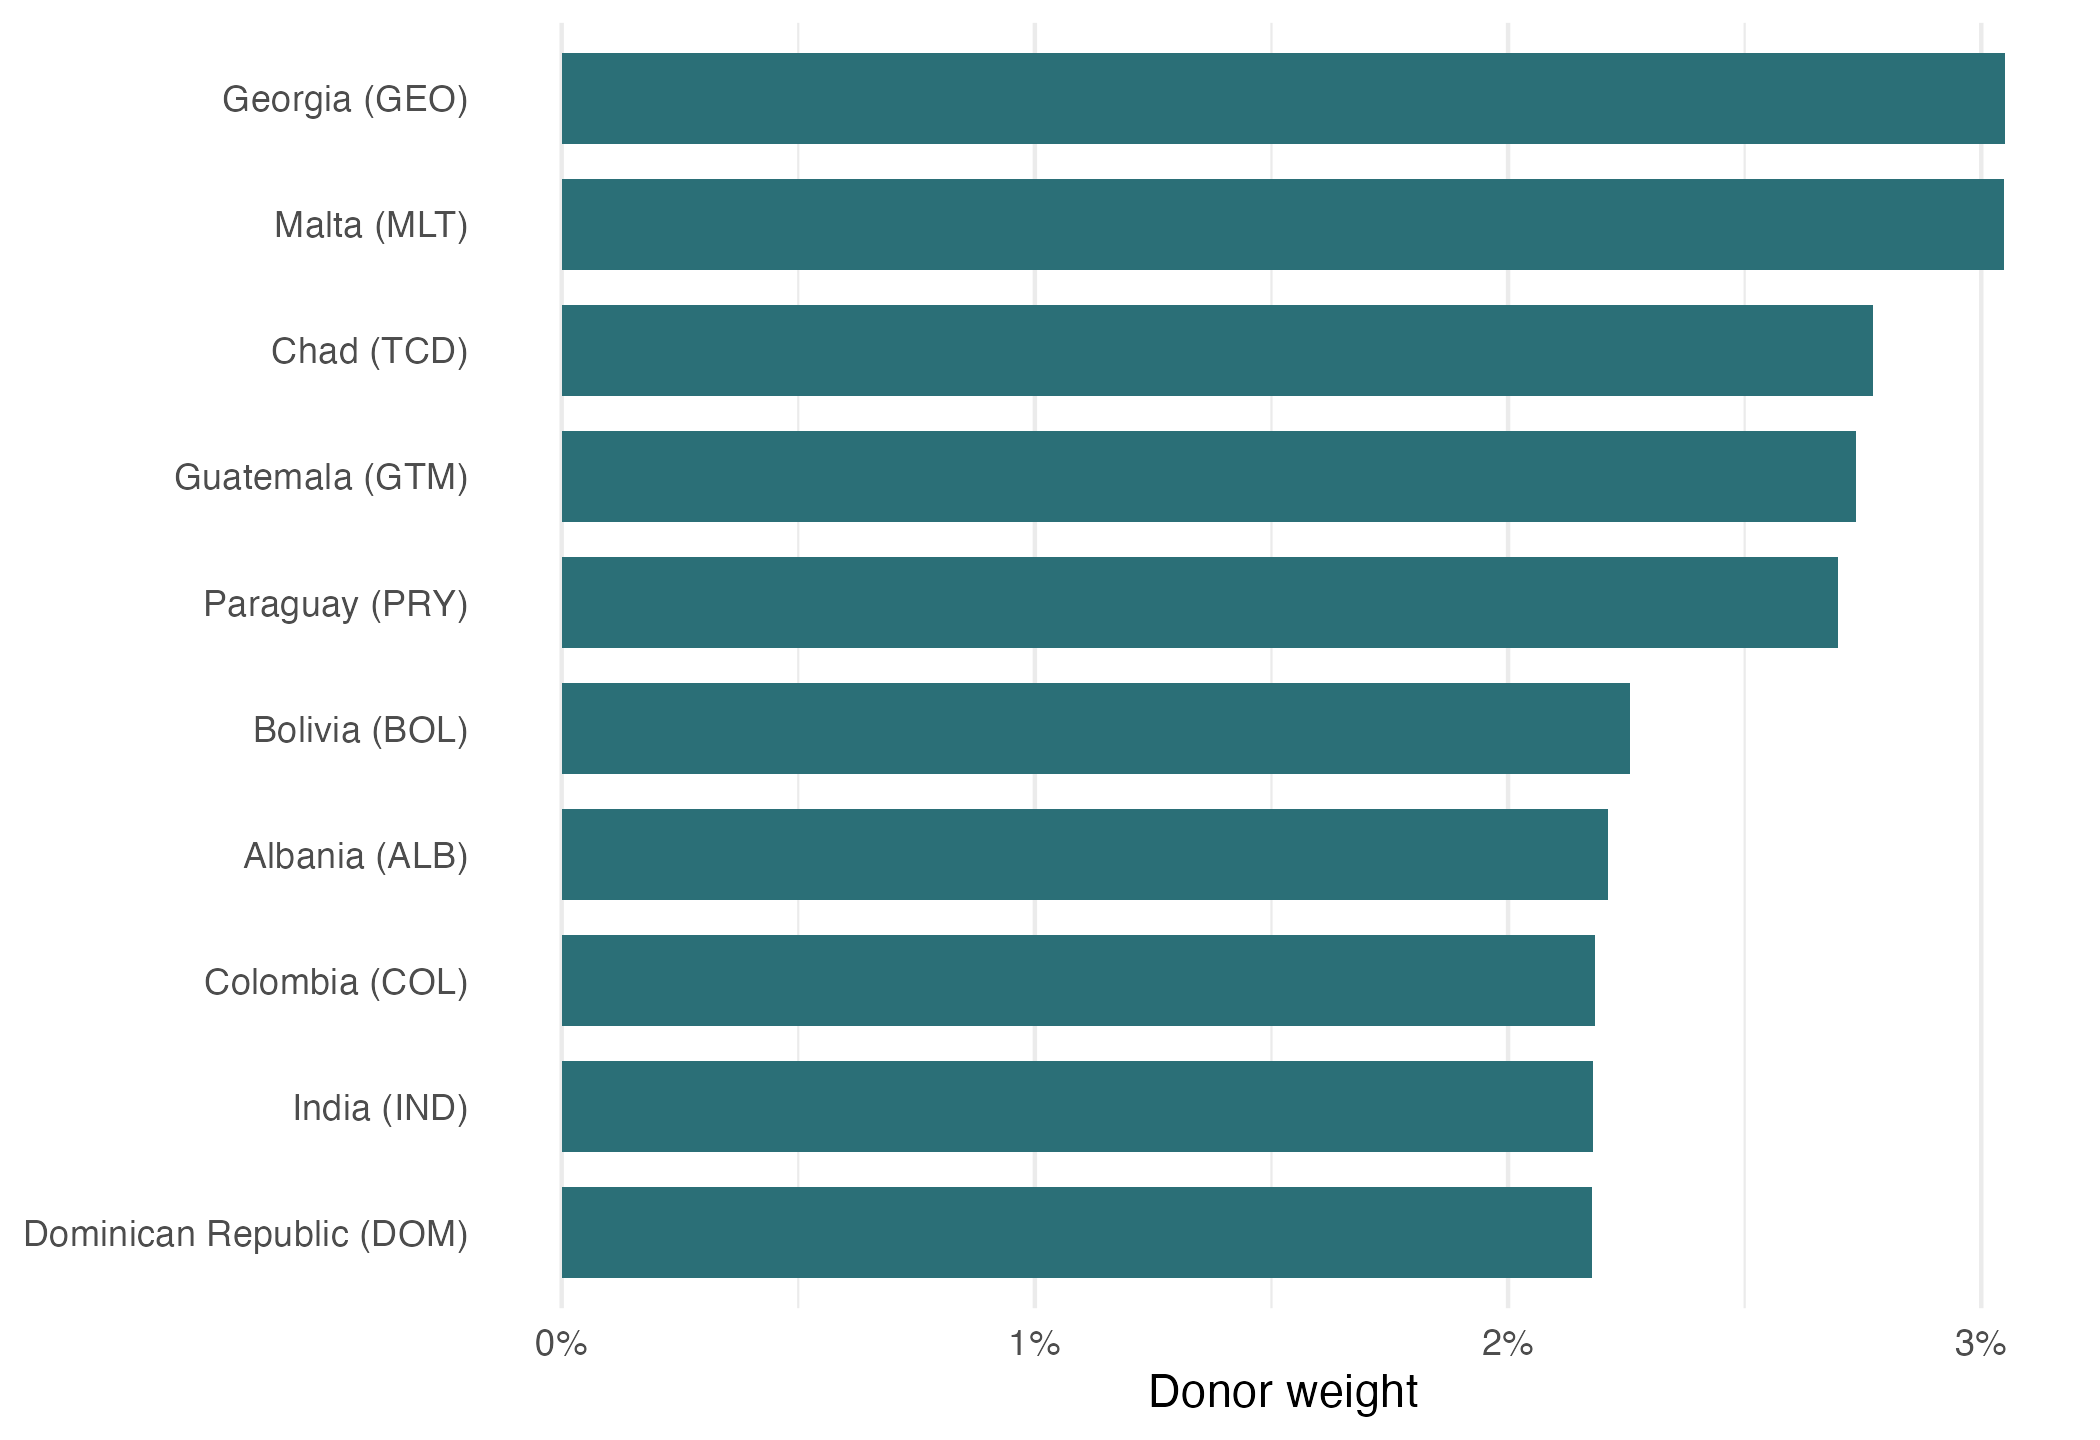
\includegraphics[width=0.9\linewidth]{quality_reports/china_demand_shock_rank_threshold/figure_brazil_sdid_predetermined_core_weights} \caption{Ten largest donor weights contributing to the synthetic control in the Brazilian SDiD model. Note: Synthetic-control unit weights, normalized over the full donor pool rather than only over the displayed donors. Window: pre-treatment period ending in 2008.}\label{fig:plot-weights}
\end{figure}

We also fit a model for a donor pool of Latin American states (excluding Caribbean countries), which is substantively attractive because the donor countries are regionally closer to Brazil. This regional donor pool is a sensitivity check rather than the preferred specification: the main design seeks a pre-treatment synthetic counterfactual with adequate donor support and fit, while the Latin American pool is much smaller.

\begin{figure}[H]
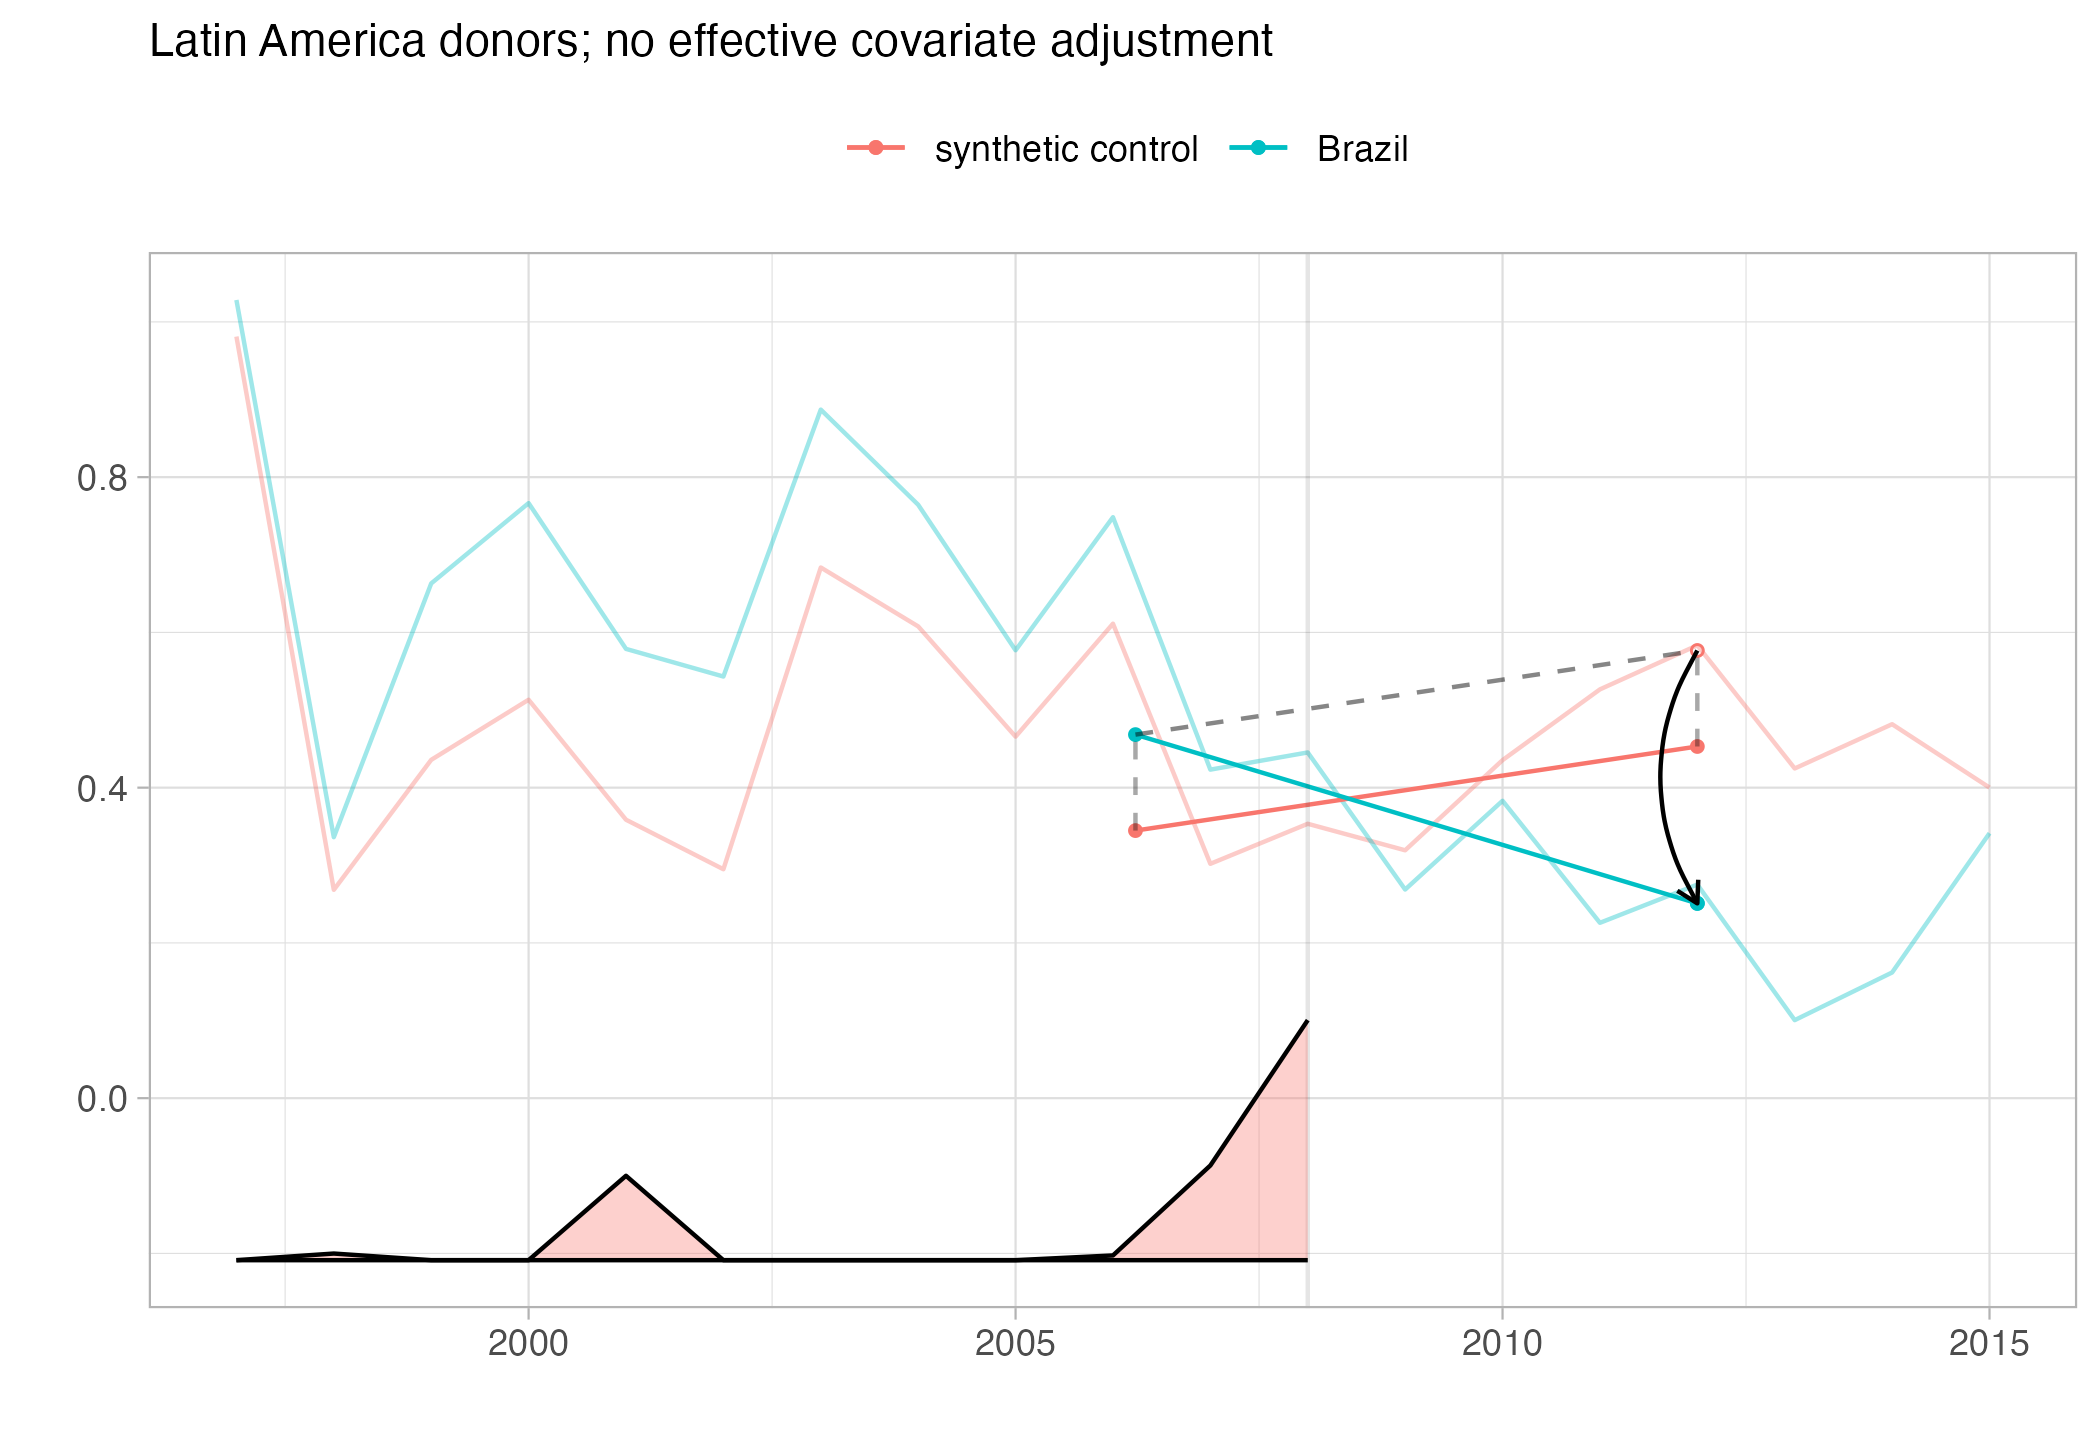
\includegraphics[width=0.95\linewidth]{quality_reports/china_demand_shock_rank_threshold/figure_brazil_sdid_predetermined_core_latam_fit} \caption{SDiD fit with a Latin American donor pool, estimated without covariates. Note: Absolute UNGA ideal-point distance to China. SE: not recomputed for this point-estimate sensitivity. Window: 1997-2015 annual series.}\label{fig:plot-latam}
\end{figure}

With the same absence of covariates, the Latin America donor-pool estimate has the same sign and a somewhat larger magnitude: -0.33, compared with -0.27 in the global donor pool. The regional pool has only 19 donors and a slightly higher intercept-adjusted pre-treatment RMSPE (0.069 versus 0.058). Because its placebo SE was not recomputed, this is a point-estimate sensitivity check. It supports stability of the negative direction but is not an independent inferential result.

\subsection{Cross-Country Robustness: Duration Thresholds}\label{cross-country-robustness-duration-thresholds}

The main cross-country estimate uses a five-year durability threshold because the theory concerns status that persists long enough to become politically usable. Table \ref{tab:cross-country-duration-table} reports the same goods-only IFE design under three- and seven-year thresholds, along with the clean single-entry robustness sample. The estimates remain negative across the restricted-risk-set rows, though precision varies with treated-unit support.

\begin{table}[H]
\centering
\caption{\label{tab:cross-country-duration-table}Duration-threshold robustness for goods-only China top export-destination status.}
\centering
\resizebox{\ifdim\width>\linewidth\linewidth\else\width\fi}{!}{
\fontsize{7}{9}\selectfont
\begin{threeparttable}
\begin{tabular}[t]{llccccccc}
\toprule
Minimum duration & Specification & ATT & SE & 95\% CI & p-value & Units (T/C) & Treated periods & r*\\
\midrule
3 & Status-current, restricted risk set & -0.113 & 0.041 & {}[-0.193, -0.034] & 0.005 & 39/126 & 477 & 2\\
3 & Clean single-entry robustness & -0.121 & 0.041 & {}[-0.202, -0.040] & 0.003 & 26/126 & 332 & 2\\
5 & Status-current, restricted risk set & -0.101 & 0.039 & {}[-0.177, -0.024] & 0.010 & 35/126 & 440 & 2\\
5 & Clean single-entry robustness & -0.122 & 0.041 & {}[-0.202, -0.042] & 0.003 & 25/126 & 329 & 2\\
7 & Status-current, restricted risk set & -0.094 & 0.040 & {}[-0.173, -0.016] & 0.019 & 31/126 & 411 & 2\\
\addlinespace
7 & Clean single-entry robustness & -0.122 & 0.042 & {}[-0.205, -0.039] & 0.004 & 23/126 & 318 & 2\\
\bottomrule
\end{tabular}
\begin{tablenotes}
\item \textit{Note: } 
\item ATT in absolute UNGA ideal-point distance to China; lower values indicate convergence toward China. SE: bootstrap with 10,000 replications. Window: goods-only ITPD-E rank metric. The restricted-risk-set rows retain clean pre-entry non-China-top years and qualifying treated years. The clean single-entry rows additionally keep only treated countries with one observed qualifying China-top period.
\end{tablenotes}
\end{threeparttable}}
\end{table}

\subsection{Cross-Country Sample Audit: Goods-Only Treatment Coding}\label{cross-country-sample-audit-goods-only-treatment-coding}

The revised rank metric excludes services before partner ranks are computed. Table \ref{tab:cross-country-sector-table} documents the ITPD-E broad-sector filter. Table \ref{tab:cross-country-audit-table} then summarizes how the five-year goods-only rule classifies countries in the UNGA/trade panel.

\begin{table}[H]
\centering
\caption{\label{tab:cross-country-sector-table}ITPD-E sector filter used to construct the goods-only China top export-destination metric.}
\centering
\fontsize{8}{10}\selectfont
\begin{tabular}[t]{lrrl}
\toprule
Broad sector & Raw rows & Positive-trade rows & Included in rank metric\\
\midrule
Agriculture & 7331458 & 2484549 & Yes\\
Manufacturing & 71208330 & 28203707 & Yes\\
Mining and Energy & 1205032 & 416413 & Yes\\
Services & 1002558 & 519520 & No\\
\bottomrule
\end{tabular}
\end{table}

\begin{table}[H]
\centering
\caption{\label{tab:cross-country-audit-table}Country-level sample audit for the five-year goods-only China top export-destination rule.}
\centering
\fontsize{8}{10}\selectfont
\begin{threeparttable}
\begin{tabular}[t]{lr}
\toprule
Role & Countries\\
\midrule
Excluded: no clean observed prior non-China-top year & 1\\
Excluded: pre-2000 China-top entry & 2\\
Excluded: short China-top periods & 26\\
Never-China-top controls & 128\\
Qualifying treated countries & 35\\
\bottomrule
\end{tabular}
\begin{tablenotes}
\item \textit{Note: } 
\item The audit uses the goods-only rank metric and classifies countries before the estimator-specific screen for minimum untreated support. Country counts are therefore a coding audit, not a replacement for the treated/control counts in the estimation table.
\end{tablenotes}
\end{threeparttable}
\end{table}

\subsection{Public Cue and Recoverability Audit}\label{public-cue-and-recoverability-audit}

The cross-country media and source audit is used only to discipline the mechanism interpretation. It does not redefine the treatment. The treatment remains durable status in which China is the country's top goods-export destination; the audit asks whether public or official rank language is recoverable around entry and whether non-recovery should be read as meaningful silence. Table \ref{tab:ex-top1-recoverability-audit} therefore separates observed China status cues, displaced-incumbent recoverability, and metric caveats. Negative cases are interpreted as recoverability diagnostics, not as proof that the status cue was absent.

\begingroup\fontsize{7}{9}\selectfont

\begin{ThreePartTable}
\begin{TableNotes}
\item \textit{Note: } 
\item The table is built from the supplemental former-incumbent audit tables. The former-incumbent benchmark asks whether the export partner displaced by China was covered in recoverable local or official sources. It is a recoverability diagnostic, not a rule for coding China salience as absent.
\end{TableNotes}
\begin{longtable}[t]{lrll>{\raggedright\arraybackslash}p{4.0cm}>{\raggedright\arraybackslash}p{4.2cm}}
\caption{\label{tab:ex-top1-recoverability-audit}Recoverability and metric caveats in the former-incumbent salience audit.}\\
\toprule
Country & Entry year & China cue & Ex-\#1 benchmark & Interpretation & Caveat\\
\midrule
Solomon Islands & 2003 & unknown & unknown & Weak observation/recoverability problem & Additional local/official archive work required.\\
Philippines & 2005 & unknown & unknown & Weak observation/recoverability problem & Treatment-rank audit issue in contemporaneous sources.\\
Angola & 2007 & unknown & unknown & Weak observation/recoverability problem & Additional local/official archive work required.\\
Malaysia & 2009 & unknown & medium & Benchmark recoverable; follow up before recoding salience & Rank-definition and China/Hong Kong aggregation caveat.\\
Australia & 2010 & unknown & medium & Metric mismatch/status already salient & Australian Financial Review uses aggregate trade; not counted for export-destination uptake.\\
\addlinespace
Sierra Leone & 2012 & unknown & unknown & Weak observation/recoverability problem & Local statistics conflict with Belgium-as-incumbent.\\
Myanmar (Burma) & 2014 & unknown & unknown & Weak observation/recoverability problem & Additional local/official archive work required.\\
Gabon & 2017 & unknown & unknown & Weak observation/recoverability problem & Additional local/official archive work required.\\
Kuwait & 2018 & unknown & unknown & Weak observation/recoverability problem & Additional local/official archive work required.\\
\bottomrule
\insertTableNotes
\end{longtable}
\end{ThreePartTable}
\endgroup{}

\begin{table}[H]
\centering
\caption{\label{tab:ex-top1-australia-afr-context}Australian Financial Review context source for Australia.}
\centering
\resizebox{\ifdim\width>\linewidth\linewidth\else\width\fi}{!}{
\fontsize{7}{9}\selectfont
\begin{threeparttable}
\begin{tabular}[t]{llllll}
\toprule
Source & Date & Metric & Counted in export-destination benchmark & Raw file & Interpretation\\
\midrule
Australian Financial Review & 2009-11-09 & Australia's largest aggregate trading partner & No & data/raw/ex\_top1\_salience/AUS/2009/australian\_financial\_review/aus\_afr\_china\_trading\_partner\_2009.html & DO\_NOT\_COUNT: broad trade-partner metric combines exports and imports, goods and services; not evidence of export-destination status. Retained as metric-mismatch and salience context.\\
\bottomrule
\end{tabular}
\begin{tablenotes}
\item \textit{Note: } 
\item The AFR item documents a broad aggregate-trading-partner cue. It is retained as context for metric mismatch and prior salience, not as evidence of newspaper uptake of the strict export-destination treatment.
\end{tablenotes}
\end{threeparttable}}
\end{table}

\clearpage

\subsection{ChatGPT Classification}\label{chatgpt-classification}

Below is the coded instruction to the ChatGPT API to classify the subjects of the headlines.

\begin{Shaded}
\begin{Highlighting}[]
\NormalTok{system\_block }\OtherTok{\textless{}{-}} \FunctionTok{paste}\NormalTok{(}
  \StringTok{\textquotesingle{}You are a Brazilian expert in International Relations and the political\textquotesingle{}}\NormalTok{,}
  \StringTok{\textquotesingle{}economy of China–Brazil relations.  Classify the subject of EACH headline\textquotesingle{}}\NormalTok{,}
  \StringTok{\textquotesingle{}when I say EACH, I mean all of them, even if repetitive or similar. Do classify **all** of them\textquotesingle{}}\NormalTok{,}
  \StringTok{\textquotesingle{}using **one** label from this list exactly as written:\textquotesingle{}}\NormalTok{,}
  \StringTok{\textquotesingle{}"diplomacy", "chinese economy", "china{-}brasil relations",\textquotesingle{}}\NormalTok{,}
  \StringTok{\textquotesingle{}"disaster and accidents", "chinese politics and policy",\textquotesingle{}}\NormalTok{,}
  \StringTok{\textquotesingle{}"sports, science, culture, other", "human rights",\textquotesingle{}}\NormalTok{,}
  \StringTok{\textquotesingle{}"china{-}brazil trade", "health".}\SpecialCharTok{\textbackslash{}n\textbackslash{}n}\StringTok{\textquotesingle{}}\NormalTok{,}
  \CommentTok{\# 13 static few{-}shot examples — leave them unchanged!}
  \StringTok{\textquotesingle{}Examples:}\SpecialCharTok{\textbackslash{}n}\StringTok{\textquotesingle{}}\NormalTok{,}
  \StringTok{\textquotesingle{}1. Presidente chinês visita o Brasil e participa de reunião com FHC {-}\textgreater{} china{-}brasil relations}\SpecialCharTok{\textbackslash{}n}\StringTok{\textquotesingle{}}\NormalTok{,}
  \StringTok{\textquotesingle{}2. Ministro chinês de Defesa faz visita oficial ao Brasil {-}\textgreater{} china{-}brasil relations}\SpecialCharTok{\textbackslash{}n}\StringTok{\textquotesingle{}}\NormalTok{,}
  \StringTok{\textquotesingle{}3. Para governo, novo câmbio chinês só beneficia Brasil no médio prazo {-}\textgreater{} china{-}brazil trade}\SpecialCharTok{\textbackslash{}n}\StringTok{\textquotesingle{}}\NormalTok{,}
  \StringTok{\textquotesingle{}4. China ultrapassa EUA como maior parceiro comercial do Brasil {-}\textgreater{} china{-}brazil trade}\SpecialCharTok{\textbackslash{}n}\StringTok{\textquotesingle{}}\NormalTok{,}
  \StringTok{\textquotesingle{}5. China vai controlar preços de alimentos e combustíveis {-}\textgreater{} chinese economy}\SpecialCharTok{\textbackslash{}n}\StringTok{\textquotesingle{}}\NormalTok{,}
  \StringTok{\textquotesingle{}6. Vendas de automóveis na China desaceleram em junho {-}\textgreater{} chinese economy}\SpecialCharTok{\textbackslash{}n}\StringTok{\textquotesingle{}}\NormalTok{,}
  \StringTok{\textquotesingle{}7. China quer devolução das relíquias Yin, patrimônio da Unesco {-}\textgreater{} sports, science, culture, other}\SpecialCharTok{\textbackslash{}n}\StringTok{\textquotesingle{}}\NormalTok{,}
  \StringTok{\textquotesingle{}8. Dinossauro encontrado na China esclarece origem das aves {-}\textgreater{} sports, science, culture, other}\SpecialCharTok{\textbackslash{}n}\StringTok{\textquotesingle{}}\NormalTok{,}
  \StringTok{\textquotesingle{}9. OMS confirma mais de 4.600 casos de gripe suína; China registra 2º caso {-}\textgreater{} health}\SpecialCharTok{\textbackslash{}n}\StringTok{\textquotesingle{}}\NormalTok{,}
  \StringTok{\textquotesingle{}10. Marinha chinesa busca "cansar" barcos japoneses em águas disputadas {-}\textgreater{} diplomacy}\SpecialCharTok{\textbackslash{}n}\StringTok{\textquotesingle{}}\NormalTok{,}
  \StringTok{\textquotesingle{}11. Acidente após casamento deixa 16 mortos na China {-}\textgreater{} disaster and accidents}\SpecialCharTok{\textbackslash{}n}\StringTok{\textquotesingle{}}\NormalTok{,}
  \StringTok{\textquotesingle{}12. Jornal chinês sai das bancas por foto da praça Tiananmen {-}\textgreater{} human rights}\SpecialCharTok{\textbackslash{}n}\StringTok{\textquotesingle{}}\NormalTok{,}
  \StringTok{\textquotesingle{}13. China é parceira estratégica contra crise econômica, diz UE {-}\textgreater{} chinese economy\textquotesingle{}}\NormalTok{,}
  \StringTok{\textquotesingle{}return as in the examples, a string with the headline and the classification\textquotesingle{}}
\NormalTok{)}
\end{Highlighting}
\end{Shaded}

The classified headline file is treated as an archived derived dataset rather than regenerated during manuscript rendering. This choice reflects the practical behavior of LLM-based coding: early runs sometimes returned incomplete classifications, altered original headlines, or used slightly inconsistent labels, which made exact matching back to the archive difficult. I therefore fixed the prompt, normalized labels, preserved the resulting classified file, and validate the coding below against an independently coded sample. The evidence in the main text is used as a headline-level salience diagnostic.

Below we provide a random sample of the headlines and the classification provided by ChatGPT.

\begin{figure}[H]
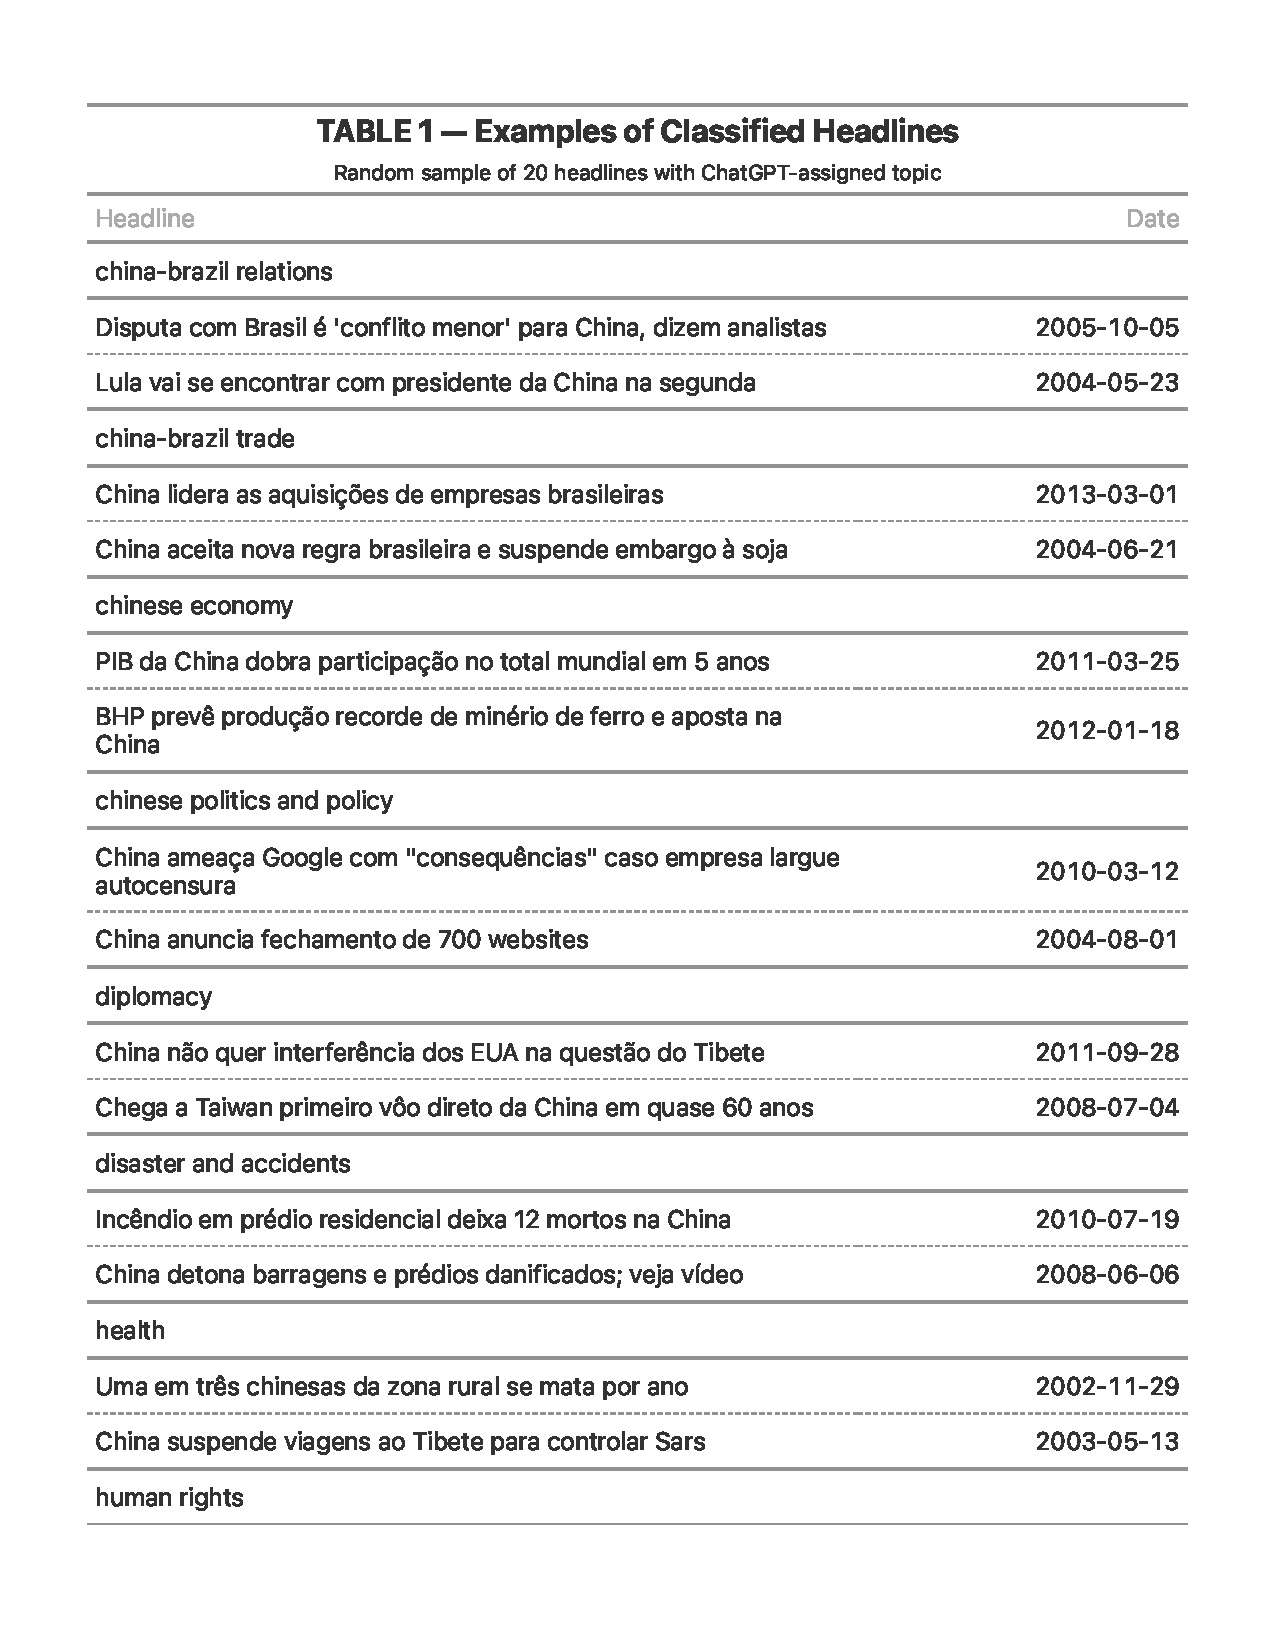
\includegraphics[width=\linewidth]{images/table1_headlines} \caption{Random sample of China-related Folha de Sao Paulo headlines and ChatGPT classifications. Note: headline text and category labels. Window: sample drawn from the 2000-2014 corpus.}\label{fig:sample-chatgpt}
\end{figure}

\subsubsection{Validation of ChatGPT Classification}\label{validation-of-chatgpt-classification}

To assess the reliability of the automated classification, one of the authors independently coded a stratified random sample of 100 headlines (with a minimum of 5 per category). Table \ref{tab:chatgpt-validation} reports the agreement rate between the ChatGPT labels and the manual coding.

\begin{table}[H]
\centering
\caption{\label{tab:chatgpt-validation}Validation of ChatGPT classification against manual coding (N = 100). Overall accuracy: 88.0 percent.}
\centering
\resizebox{\ifdim\width>\linewidth\linewidth\else\width\fi}{!}{
\fontsize{9}{11}\selectfont
\begin{threeparttable}
\begin{tabular}[t]{lccc}
\toprule
Category & N & Correct & Accuracy (\%)\\
\midrule
china-brazil trade & 6 & 6 & 100.0\\
disaster and accidents & 13 & 13 & 100.0\\
health & 6 & 6 & 100.0\\
chinese economy & 25 & 24 & 96.0\\
human rights & 8 & 7 & 87.5\\
\addlinespace
diplomacy & 12 & 10 & 83.3\\
sports, science, culture, other & 17 & 14 & 82.4\\
china-brazil relations & 5 & 4 & 80.0\\
chinese politics and policy & 8 & 4 & 50.0\\
Overall & 100 & 88 & 88.0\\
\bottomrule
\end{tabular}
\begin{tablenotes}
\item \textit{Note: } 
\item headline-level counts and accuracy (percent) by category. Window: stratified validation sample from the 2000-2014 headline corpus.
\end{tablenotes}
\end{threeparttable}}
\end{table}

The overall accuracy is 88.0 percent. The lowest agreement is in the ``chinese politics and policy'' category (50.0 percent), where several headlines were manually reclassified as ``diplomacy''. The category most central to the mechanism, ``china-brazil trade,'' achieved 100.0 percent agreement. Related bilateral categories had lower but still usable agreement: 80.0 percent for ``china-brazil relations'' and 83.3 percent for ``diplomacy.''

\subsection{Cross-Country: Goods-Only Treated Countries}\label{cross-country-goods-only-treated-countries}

Table \ref{tab:table-treated-appendix} describes the 35 treated countries in the main goods-only restricted-risk-set specification. For each country, the table reports the first qualifying China-top goods-export year and the number of treated and untreated country-years retained in the estimation panel.

\begin{table}[!h]
\centering
\caption{\label{tab:table-treated-appendix}Treated countries in the main goods-only restricted-risk-set cross-country specification.}
\centering
\resizebox{\ifdim\width>\linewidth\linewidth\else\width\fi}{!}{
\fontsize{9}{11}\selectfont
\begin{threeparttable}
\begin{tabular}[t]{llccccc}
\toprule
Country & ISO3c & Treatment year & Treated years & Pre/other untreated years & First panel year & Last panel year\\
\midrule
Sudan & SDN & 2000 & 6 & 10 & 1990 & 2005\\
Solomon Islands & SLB & 2003 & 20 & 13 & 1990 & 2022\\
South Korea & KOR & 2003 & 20 & 12 & 1991 & 2022\\
Cuba & CUB & 2004 & 18 & 14 & 1990 & 2022\\
Oman & OMN & 2004 & 19 & 13 & 1990 & 2022\\
\addlinespace
Philippines & PHL & 2005 & 18 & 15 & 1990 & 2022\\
Yemen & YEM & 2005 & 11 & 13 & 1991 & 2015\\
Mauritania & MRT & 2006 & 17 & 15 & 1990 & 2022\\
Angola & AGO & 2007 & 16 & 17 & 1990 & 2022\\
Chile & CHL & 2007 & 16 & 17 & 1990 & 2022\\
\addlinespace
Iran & IRN & 2007 & 13 & 17 & 1990 & 2019\\
Kazakhstan & KAZ & 2007 & 16 & 15 & 1992 & 2022\\
Congo - Kinshasa & COD & 2008 & 14 & 18 & 1990 & 2022\\
Japan & JPN & 2008 & 15 & 18 & 1990 & 2022\\
North Korea & PRK & 2008 & 12 & 13 & 1991 & 2019\\
\addlinespace
Thailand & THA & 2008 & 14 & 18 & 1990 & 2021\\
Australia & AUS & 2009 & 14 & 19 & 1990 & 2022\\
Brazil & BRA & 2009 & 14 & 19 & 1990 & 2022\\
Malaysia & MYS & 2009 & 14 & 19 & 1990 & 2022\\
South Africa & ZAF & 2009 & 14 & 15 & 1994 & 2022\\
\addlinespace
Peru & PER & 2010 & 13 & 20 & 1990 & 2022\\
Turkmenistan & TKM & 2010 & 13 & 18 & 1992 & 2022\\
Congo - Brazzaville & COG & 2011 & 12 & 18 & 1990 & 2022\\
Zimbabwe & ZWE & 2011 & 7 & 21 & 1990 & 2017\\
Russia & RUS & 2012 & 11 & 20 & 1992 & 2022\\
\addlinespace
Sierra Leone & SLE & 2012 & 11 & 22 & 1990 & 2022\\
New Zealand & NZL & 2013 & 10 & 23 & 1990 & 2022\\
Saudi Arabia & SAU & 2013 & 10 & 23 & 1990 & 2022\\
Uruguay & URY & 2013 & 10 & 23 & 1990 & 2022\\
Eritrea & ERI & 2014 & 9 & 21 & 1993 & 2022\\
\addlinespace
Myanmar (Burma) & MMR & 2014 & 9 & 24 & 1990 & 2022\\
Indonesia & IDN & 2016 & 7 & 25 & 1990 & 2022\\
Equatorial Guinea & GNQ & 2017 & 6 & 18 & 1995 & 2022\\
Gabon & GAB & 2017 & 6 & 27 & 1990 & 2022\\
Kuwait & KWT & 2018 & 5 & 28 & 1990 & 2022\\
\bottomrule
\end{tabular}
\begin{tablenotes}
\item \textit{Note: } 
\item Ranks are computed from goods exports only. The restricted risk set keeps clean pre-entry non-China-top years and qualifying treated years for treated countries. Treatment year is the first retained year of a qualifying China-top goods-export period.
\end{tablenotes}
\end{threeparttable}}
\end{table}

\end{document}
